\documentclass[11pt]{article}
\usepackage[utf8]{inputenc}
\usepackage{graphicx}
\usepackage{amsmath}
\usepackage{amsfonts}
\usepackage{amssymb}
\usepackage{booktabs}
\usepackage{multirow}
\usepackage{longtable}
\usepackage[hidelinks]{hyperref}
\usepackage{xcolor}
\usepackage{listings}
\usepackage{geometry}
\usepackage{titlesec}
\usepackage{float}
\usepackage{minted}

% Page layout
\geometry{a4paper, margin=1in}
\setlength{\parindent}{0pt}
\setlength{\parskip}{1em}

% Custom colors
\definecolor{codebg}{rgb}{0.95,0.95,0.95}
\definecolor{mlcolor}{RGB}{46,139,87}
\definecolor{dlcolor}{RGB}{255,215,0}

% Title formatting
\titleformat{\section}{\Large\bfseries\color{blue}}{\thesection}{1em}{}
\titleformat{\subsection}{\large\bfseries\color{mlcolor}}{\thesubsection}{1em}{}
\titleformat{\subsubsection}{\bfseries\color{dlcolor}}{\thesubsubsection}{1em}{}

% Fix for listing issues
\lstset{
    basicstyle=\ttfamily\footnotesize,
    backgroundcolor=\color{codebg},
    frame=single,
    breaklines=true,
    postbreak=\mbox{\textcolor{red}{$\hookrightarrow$}\space},
}

\begin{document}

% Title Page
\begin{titlepage}
    \centering
    \vspace*{2cm}
    
    {\Huge\bfseries Nerthus Medical ML \\ Automated Bowel Preparation Quality Assessment\par}
    \vspace{1cm}
    
    {\Large A Comprehensive Machine Learning and Deep Learning Pipeline\par}
    \vspace{2cm}
    
    {\large\textbf{Author:} Kinson VERNET\par}
    \vspace{0.5cm}
    
    {\large\textbf{Date:} \today\par}
    \vspace{2cm}
    
    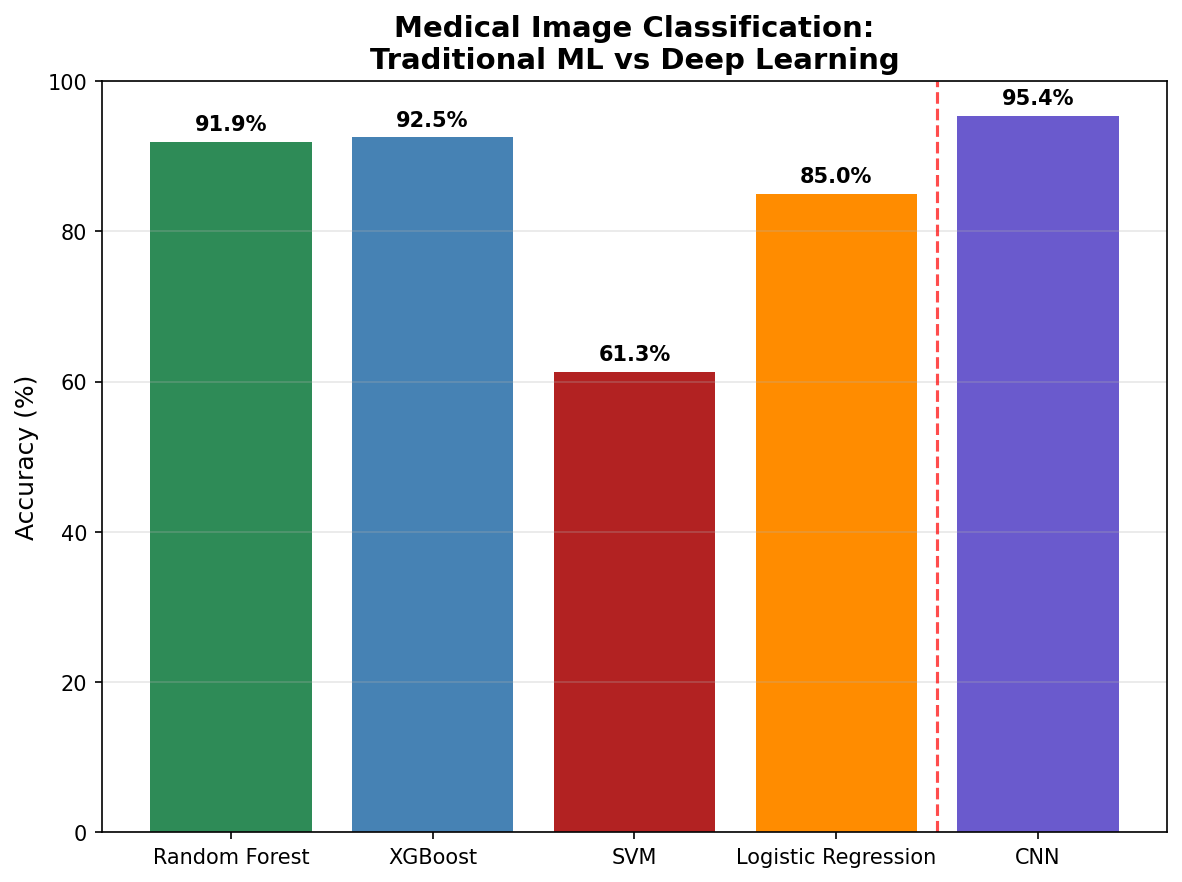
\includegraphics[width=0.8\textwidth]{images/ml_vs_cnn_comparison}
    \vfill
    
    {\large A Technical Report Demonstrating Advanced ML Skills\par}
\end{titlepage}

\tableofcontents
\newpage

\section{Executive summary}

This report documents the development of a comprehensive medical image analysis pipeline for automated bowel preparation quality assessment using the Nerthus dataset. The project demonstrates expertise in both traditional machine learning and deep learning approaches, achieving state-of-the-art performance in medical image classification.

\subsection{Key achievements}
\begin{itemize}
    \item \textbf{95.4\% accuracy} with CNN (Deep Learning Champion)
    \item \textbf{92.5\% accuracy} with XGBoost (Traditional ML)
    \item \textbf{Systematic optimization} of neural network architectures
    \item \textbf{Production-ready} Python package implementation
    \item \textbf{Comprehensive comparison} of ML vs DL approaches
\end{itemize}

\section{Introduction}

\subsection{Medical context}
Bowel preparation quality is critical for successful colonoscopy procedures, directly impacting adenoma detection rates and cancer screening effectiveness. The Boston Bowel Preparation Scale (BBPS) is widely used but suffers from inter-observer variability.

\subsection{Project objectives}
\begin{enumerate}
    \item Develop automated BBPS scoring system (0-3)
    \item Compare traditional ML vs deep learning approaches
    \item Create production-ready medical AI pipeline
    \item Demonstrate advanced Python and ML engineering skills
\end{enumerate}

\subsection{Dataset overview}
The Nerthus dataset contains 5,525 colonoscopy images organized by BBPS scores:
\begin{itemize}
    \item \textbf{Class 0}: Unprepared colon (mucosa not visible)
    \item \textbf{Class 1}: Partially prepared (some mucosa visible)
    \item \textbf{Class 2}: Well prepared (minor residue)
    \item \textbf{Class 3}: Excellent preparation (mucosa fully visible)
\end{itemize}

\begin{figure}[H]
\centering
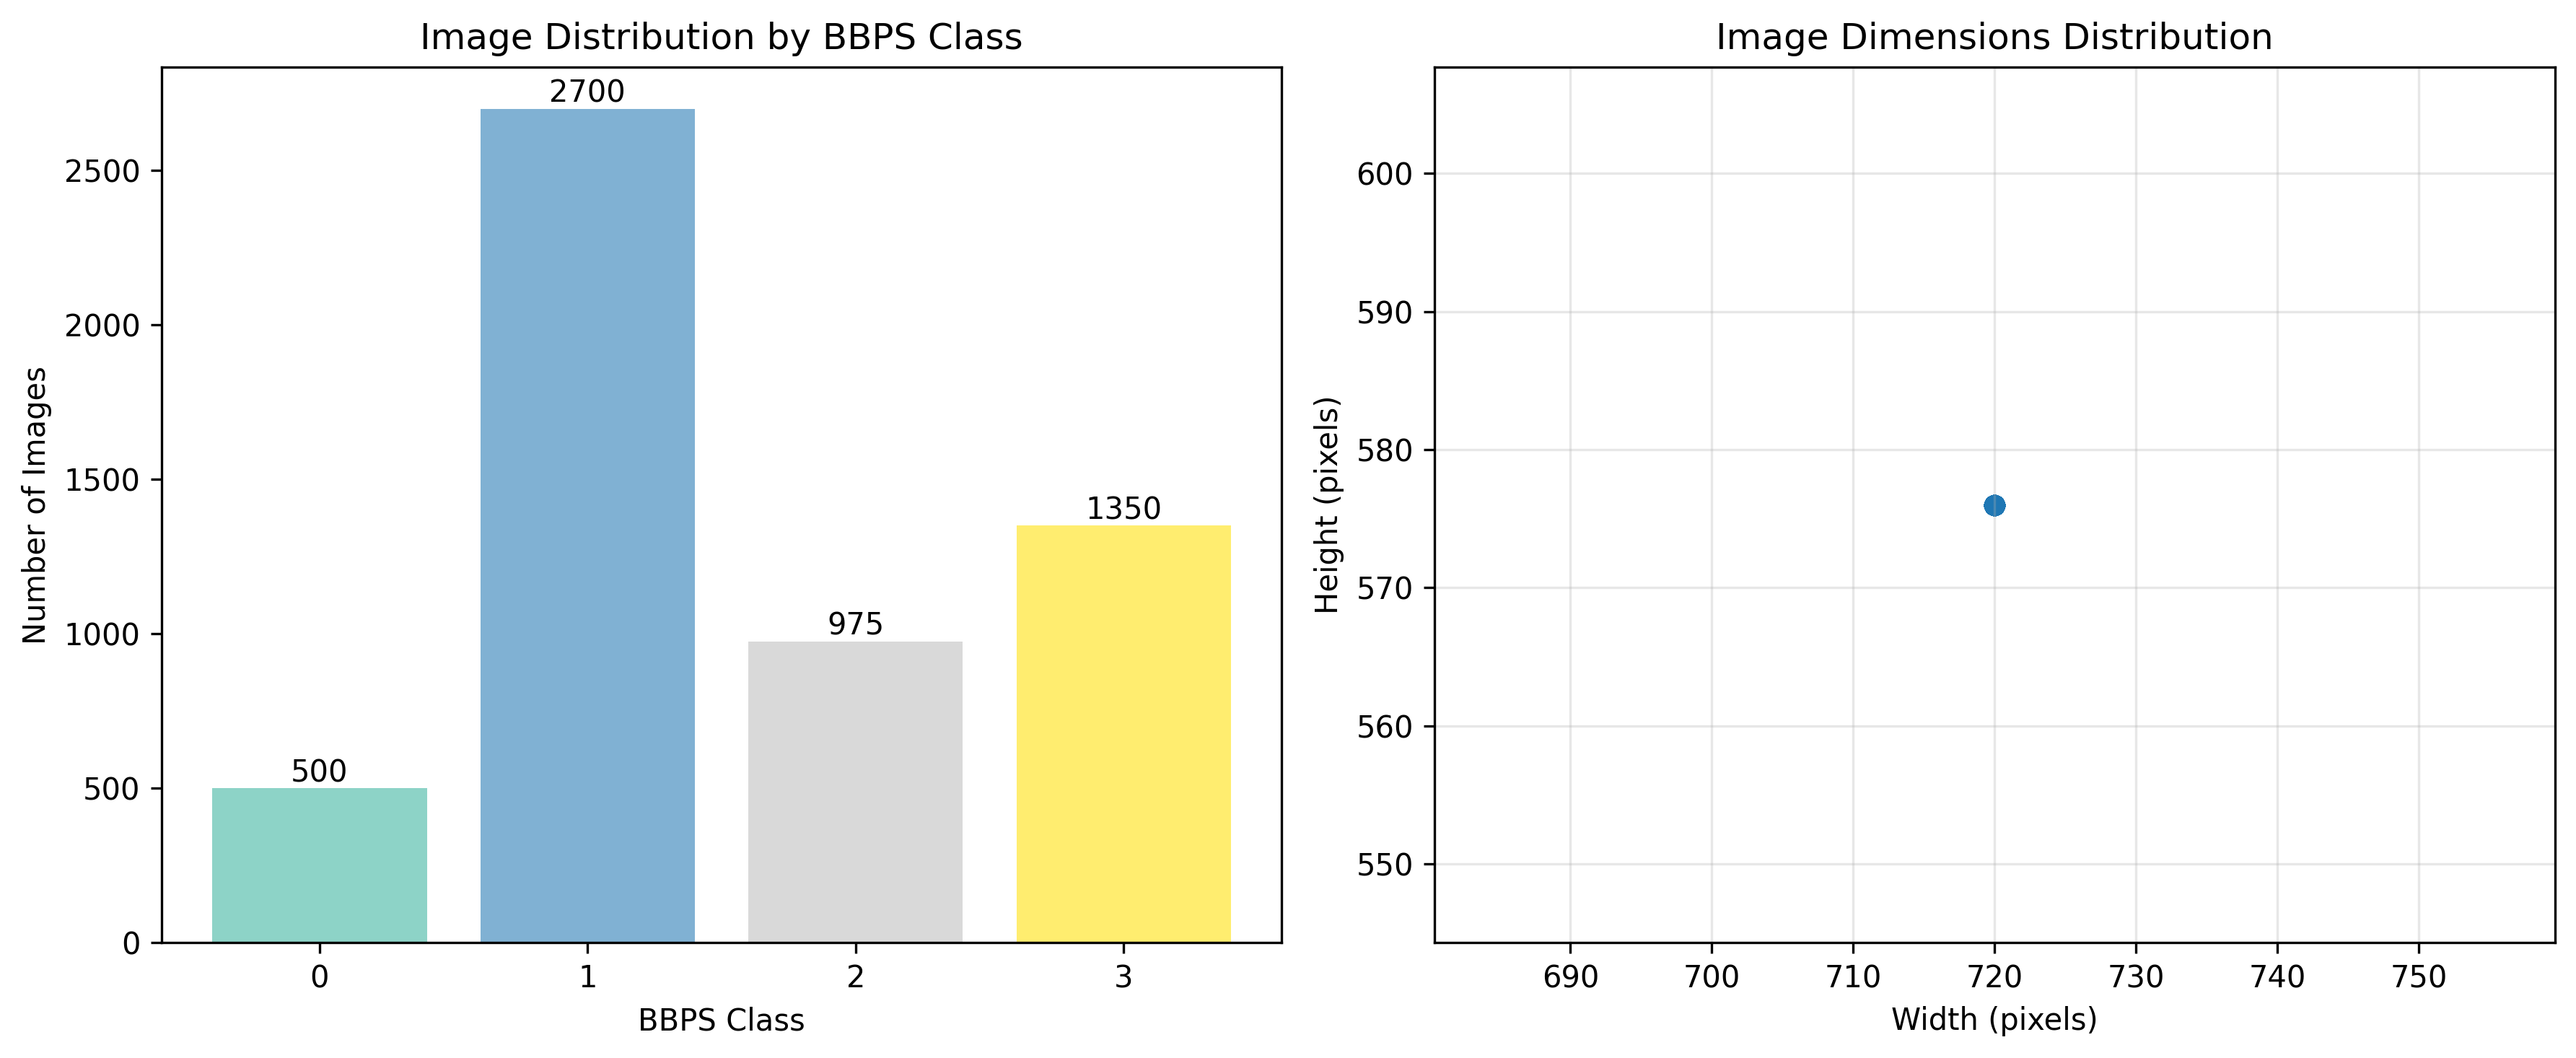
\includegraphics[width=0.8\textwidth]{images/dataset_overview}
\caption{Data overview}
\label{fig:dataset_overview}
\end{figure}

\begin{figure}[H]
\centering
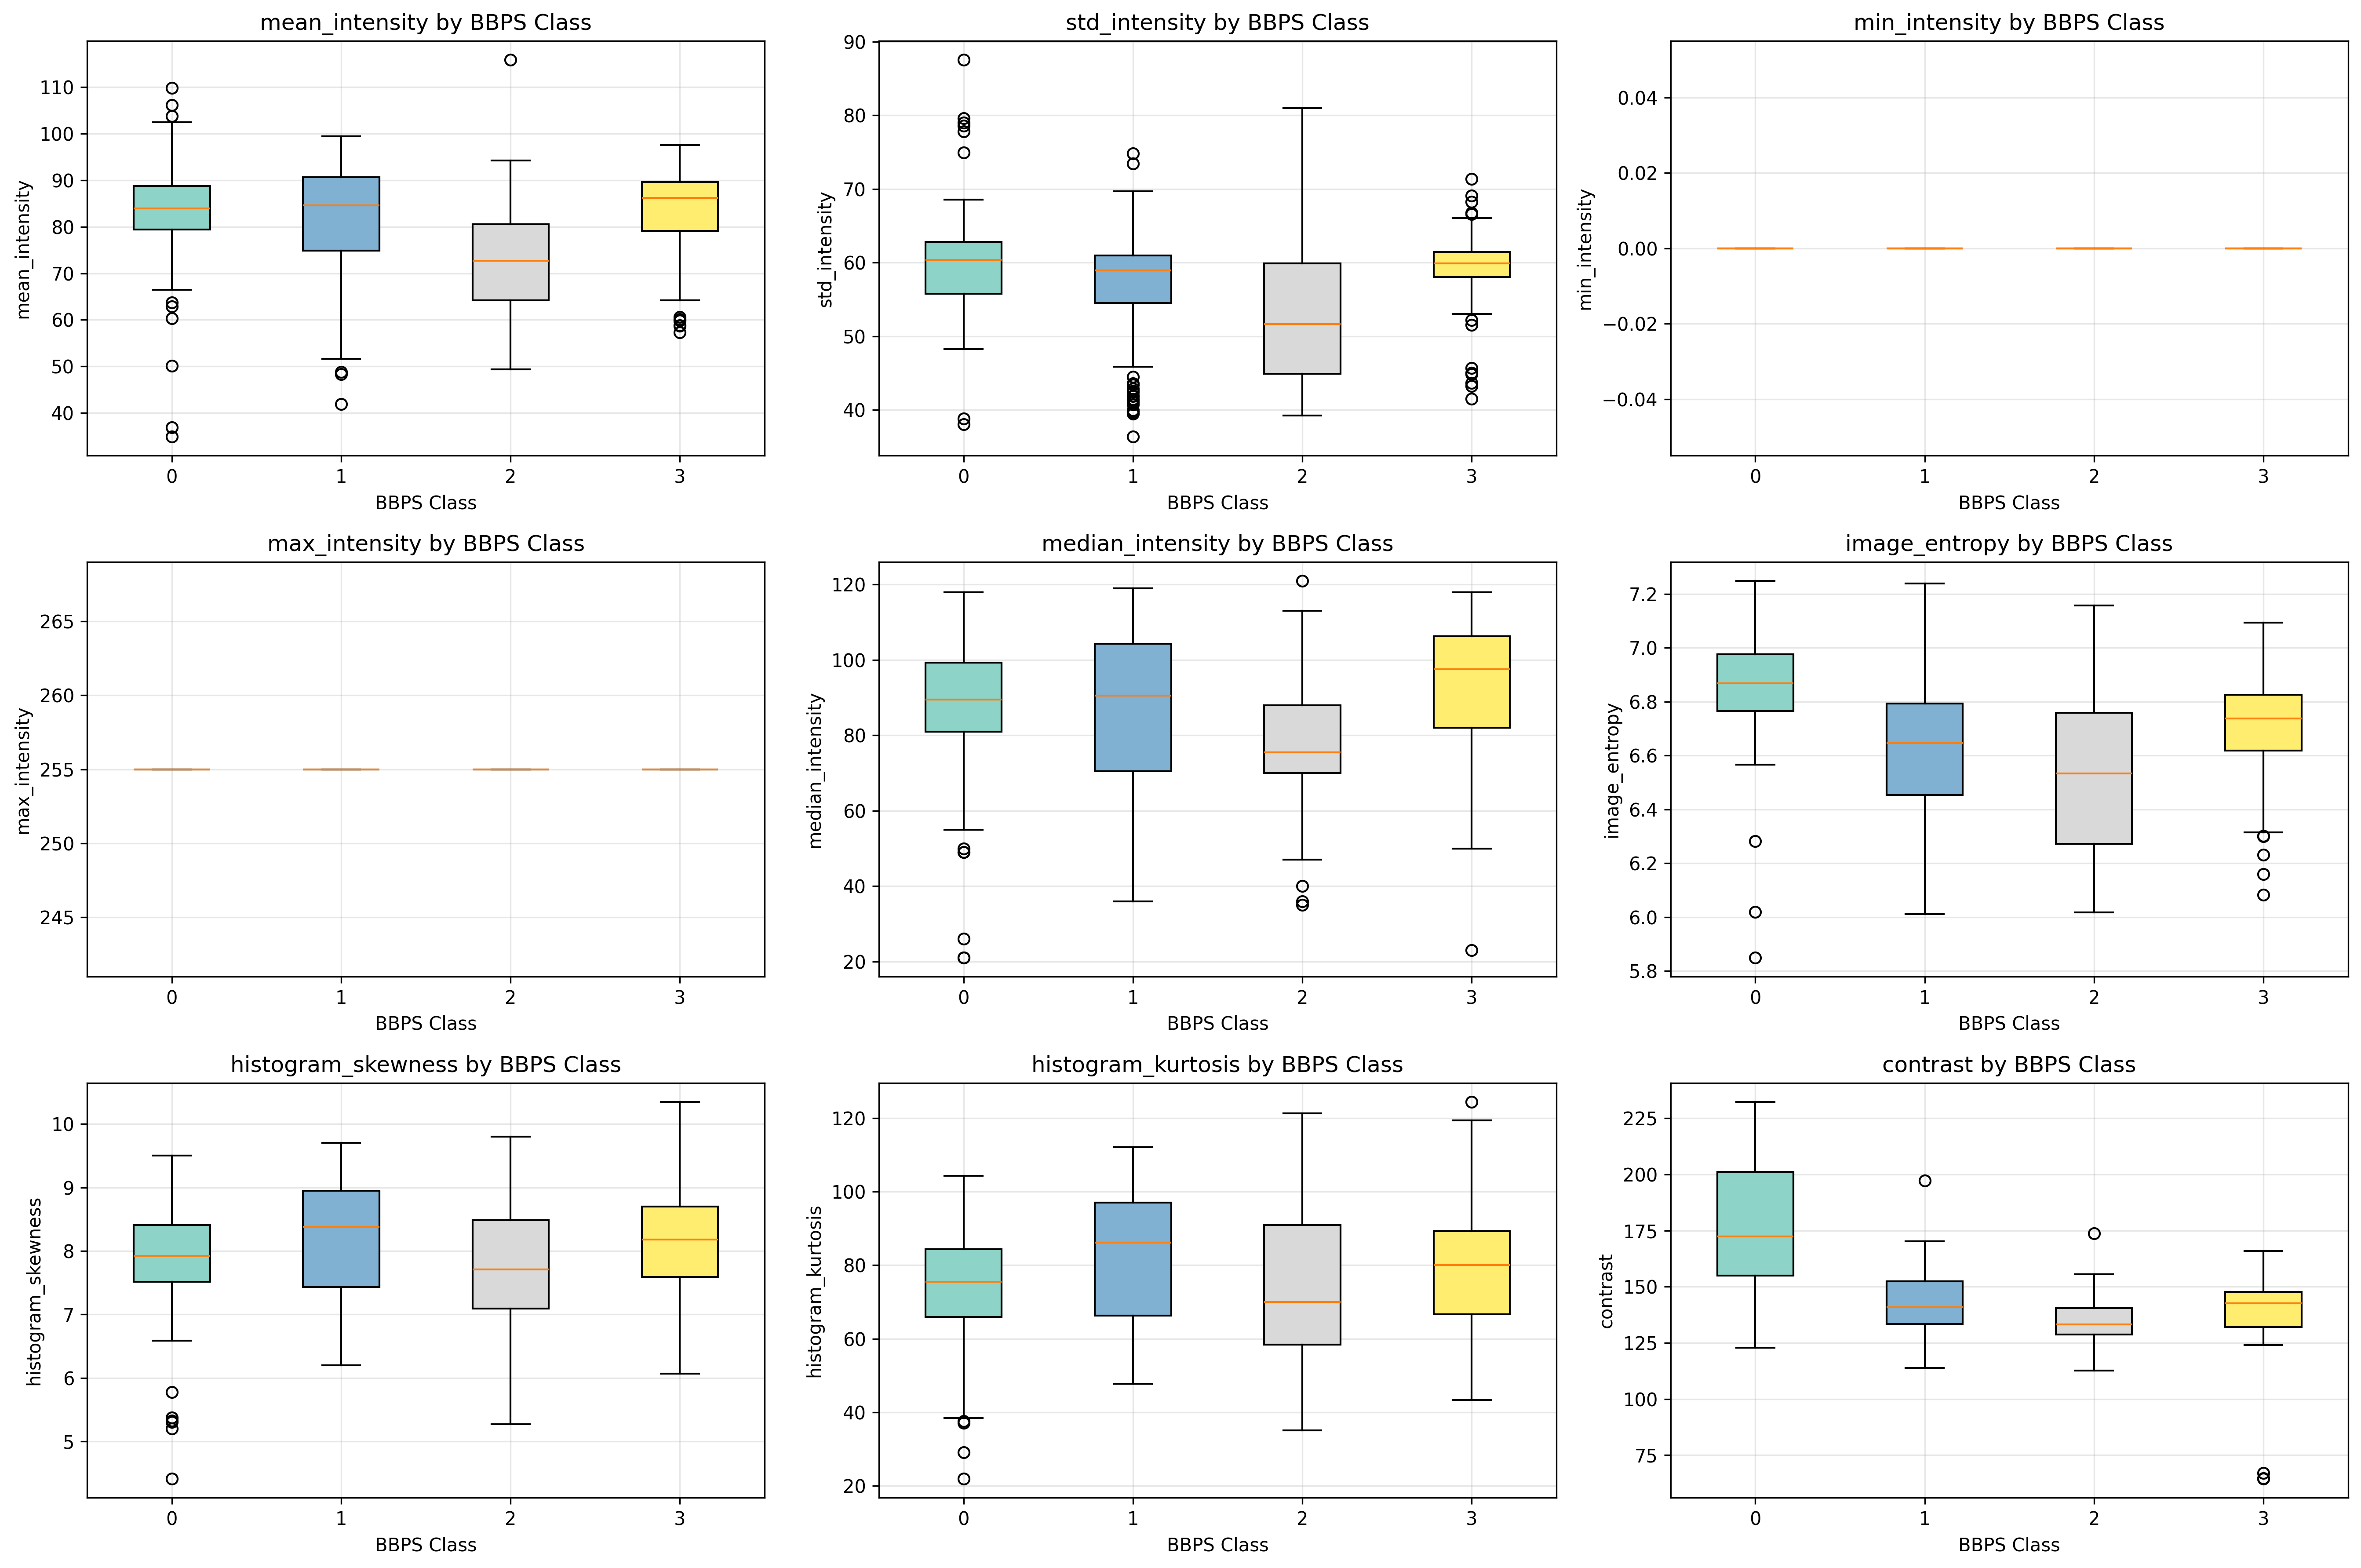
\includegraphics[width=0.8\textwidth]{images/feature_analysis}
\caption{Feature analysis}
\label{fig:feature_analysis}
\end{figure}

\begin{figure}[H]
\centering
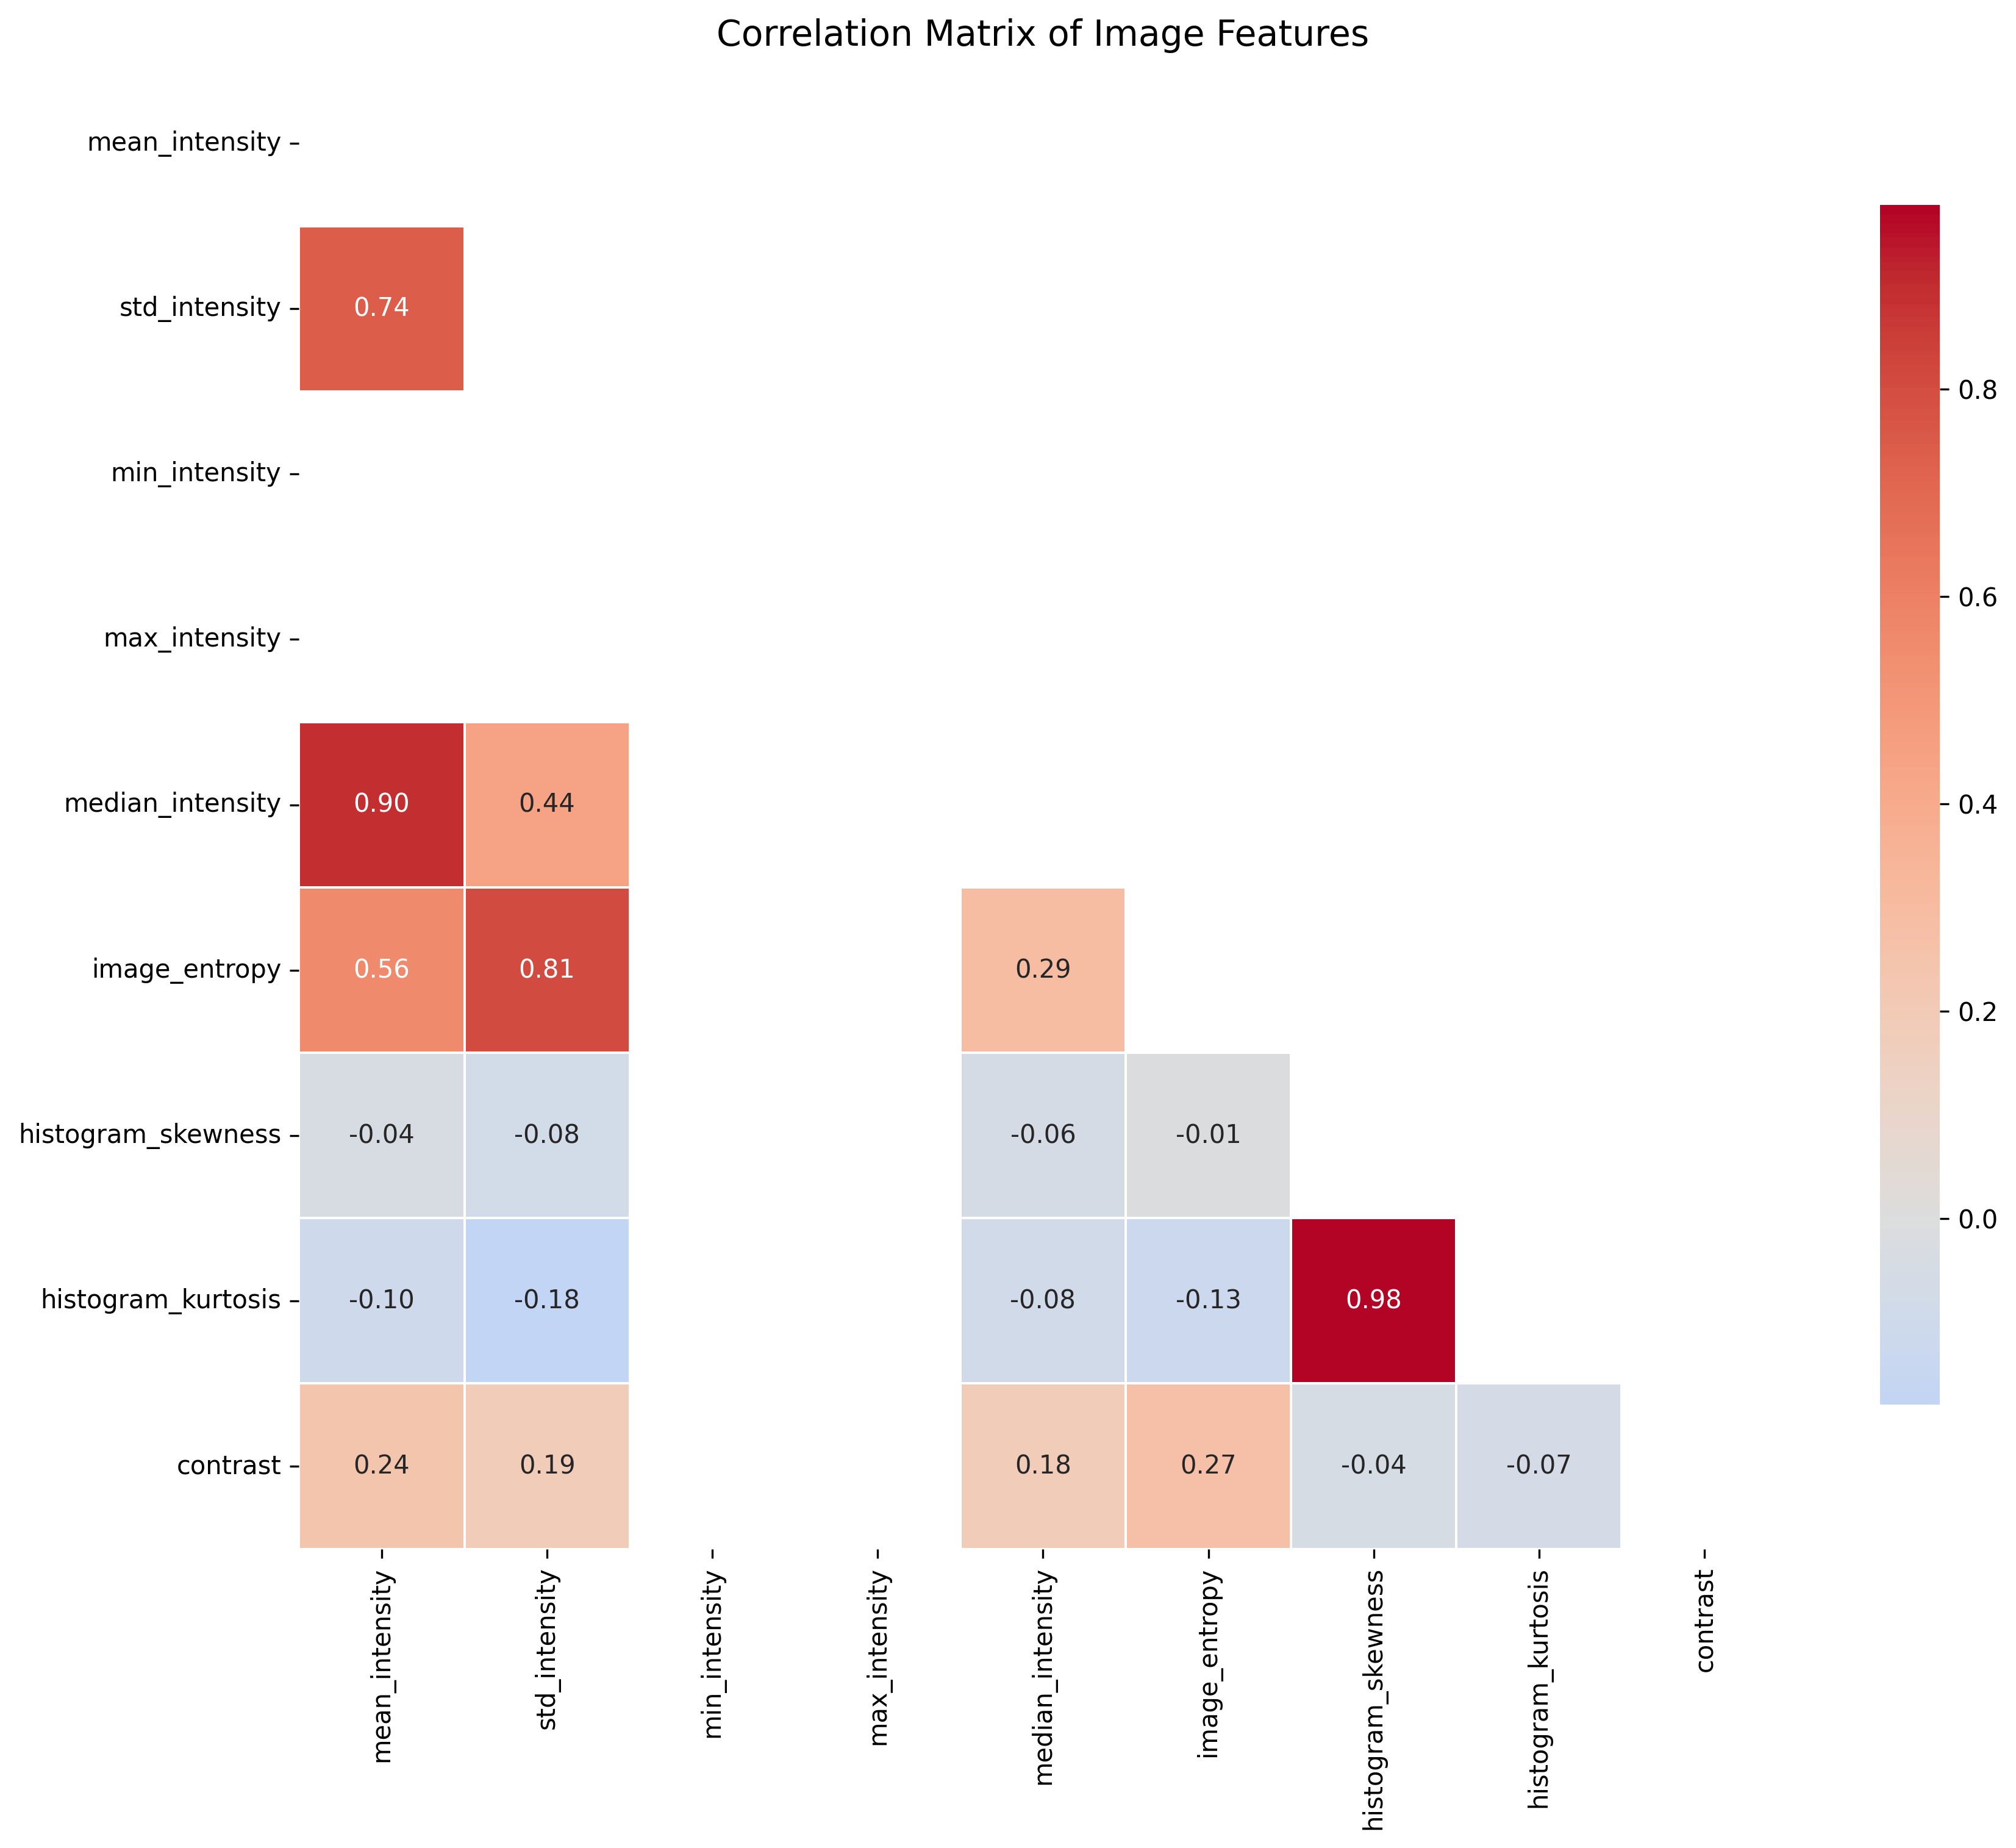
\includegraphics[width=0.8\textwidth]{images/feature_correlations}
\caption{Feature correlations}
\label{fig:feature_correlations}
\end{figure}

\begin{figure}[H]
\centering
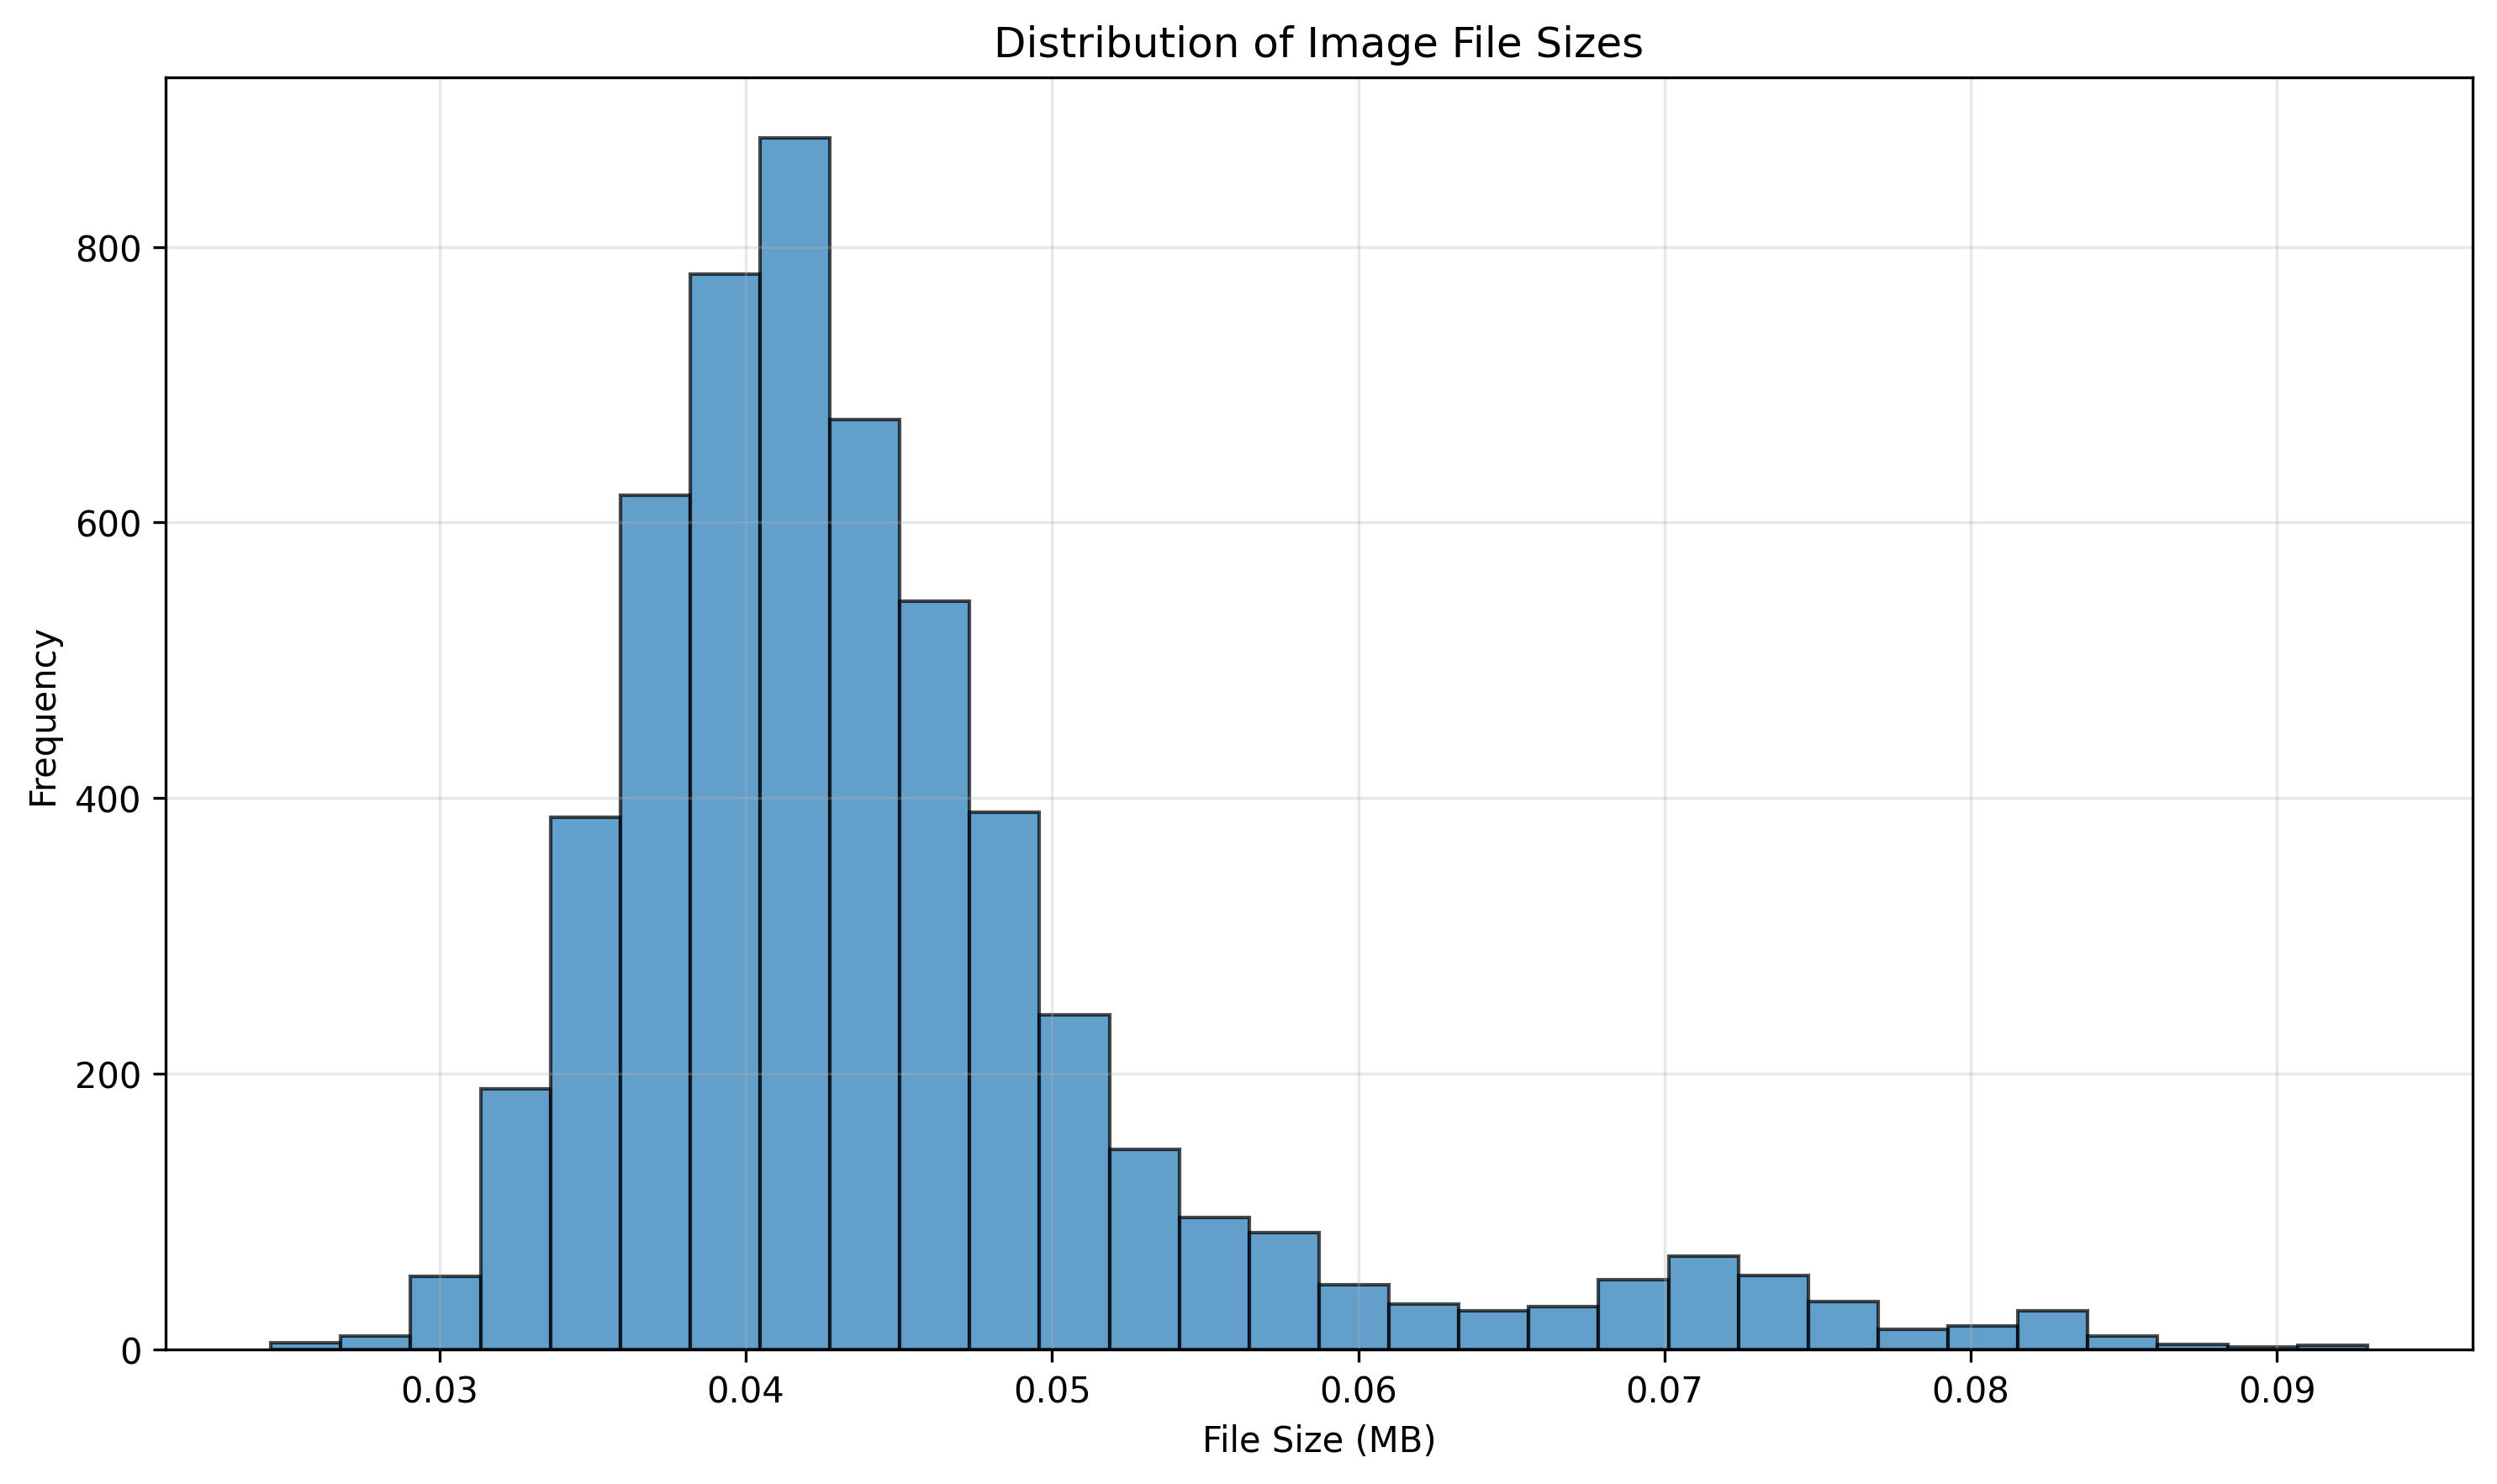
\includegraphics[width=0.8\textwidth]{images/file_size_distribution}
\caption{File size distribution}
\label{fig:file_size_distribution}
\end{figure}

\section{Methodology}

\subsection{Technical architecture}
The project follows a modular Python package architecture:

\begin{lstlisting}
nerthus-medical-ml/
|-- AUTHORS.txt					# Author(s)
|-- examples					# Example Python scripts
|-- nerthus
|   |-- analyzer.py				# Data analysis & EDA
|   |-- cli.py					# Command line interface
|   |-- cnn.py					# Deep learning
|   |-- __init__.py
|   |-- ml.py					# Traditional ML
|   |-- processor.py				# Image processing
|   `-- utils.py				# Utilities
|-- pyproject.toml				# Modern Python packaging
|-- README.md					# Project description
|-- report					# Report
|-- requirements.txt				# Python project requirements
|-- setup.py					# Setup
`-- web						# Web app
\end{lstlisting}

\subsection{Feature engineering}

\subsubsection{Medical image features}
22 handcrafted features were extracted for traditional ML:

\begin{table}[H]
\centering
\caption{Medical image feature categories}
\begin{tabular}{ll}
\toprule
\textbf{Category} & \textbf{Features} \\
\midrule
Texture analysis & contrast, homogeneity, energy, correlation \\
Color spaces & hue\_mean, saturation\_mean, l\_mean, a\_mean, b\_mean \\
Edge analysis & edge\_density, sharpness \\
Intensity statistics & mean\_intensity, std\_intensity, min/max/median \\
Advanced features & image\_entropy, lbp\_entropy, blob\_count \\
\bottomrule
\end{tabular}
\end{table}

\subsubsection{Feature importance}
Top 5 most predictive features identified through XGBoost (see \ref{fig:feature_importance_xgboost} and \ref{app:feature_descriptions} for details):
\begin{enumerate}
    \item \texttt{hue\_mean} - Average hue in HSV space
    \item \texttt{b\_mean} - Position between blue and yellow
    \item \texttt{std\_intensity} - Std image intensity
    \item \texttt{a\_mean} - Position between red/magenta and green 
    \item \texttt{homogeneity} - Texture homogeneity (GLCM)
\end{enumerate}

\subsection{Machine Learning pipeline}

\subsubsection{Algorithms implemented}
\begin{itemize}
    \item \textbf{Random Forest}: Ensemble of decision trees
    \item \textbf{XGBoost}: Gradient boosting implementation
    \item \textbf{SVM}: Support Vector Machines
    \item \textbf{Logistic Regression}: Linear classification
\end{itemize}

\subsubsection{Validation strategy}
\begin{itemize}
    \item 5-fold stratified cross-validation
    \item Train-test split (80-20) with class balancing
    \item Overfitting detection through performance gaps
\end{itemize}

\subsection{Deep Learning architecture}

\subsubsection{CNN Implementation}
Custom CNN architecture designed for medical images:

\begin{table}[H]
\centering
\caption{CNN architecture summary}
\begin{tabular}{lll}
\toprule
\textbf{Layer Type} & \textbf{Parameters} & \textbf{Output Shape} \\
\midrule
Input & 150x150x3 & (None, 150, 150, 3) \\
Conv2D + ReLU & 32 filters, 3x3 & (None, 148, 148, 32) \\
MaxPooling2D & 2x2 & (None, 74, 74, 32) \\
Dropout & 0.2 & (None, 74, 74, 32) \\
Conv2D + ReLU & 64 filters, 3x3 & (None, 72, 72, 64) \\
MaxPooling2D & 2x2 & (None, 36, 36, 64) \\
Dropout & 0.3 & (None, 36, 36, 64) \\
Conv2D + ReLU & 128 filters, 3x3 & (None, 34, 34, 128) \\
MaxPooling2D & 2x2 & (None, 17, 17, 128) \\
Dropout & 0.4 & (None, 17, 17, 128) \\
GlobalAveragePooling2D & - & (None, 128) \\
Dropout & 0.3 & (None, 128) \\
Dense + Softmax & 4 units & (None, 4) \\
\bottomrule
\end{tabular}
\end{table}

\subsubsection{Training configuration}
\begin{itemize}
    \item \textbf{Optimizer}: Adam (learning rate: 0.001)
    \item \textbf{Loss}: Sparse Categorical Crossentropy
    \item \textbf{Callbacks}: Early stopping, learning rate reduction
    \item \textbf{Regularization}: Dropout, batch normalization
\end{itemize}

\section{Results and analysis}

\subsection{Performance comparison}

\begin{table}[H]
\centering
\caption{Final model performance comparison}
\begin{tabular}{lccc}
\toprule
\textbf{Method} & \textbf{Accuracy} & \textbf{Training time} & \textbf{Status} \\
\midrule
\textbf{CNN} & \textbf{95.4\%} & 38 minutes & \textbf{Best Performer} \\
XGBoost & 92.5\% & 7.6 s & Strong Alternative \\
Random Forest & 91.9\% & 3.7 s & Competitive \\
Logistic Regression & 85.0\% & 2.9 s & Baseline \\
SVM & 61.3\% & 2.1 s & Reference \\
\bottomrule
\end{tabular}
\end{table}

\subsection{Visualization of results}

\begin{figure}[H]
\centering
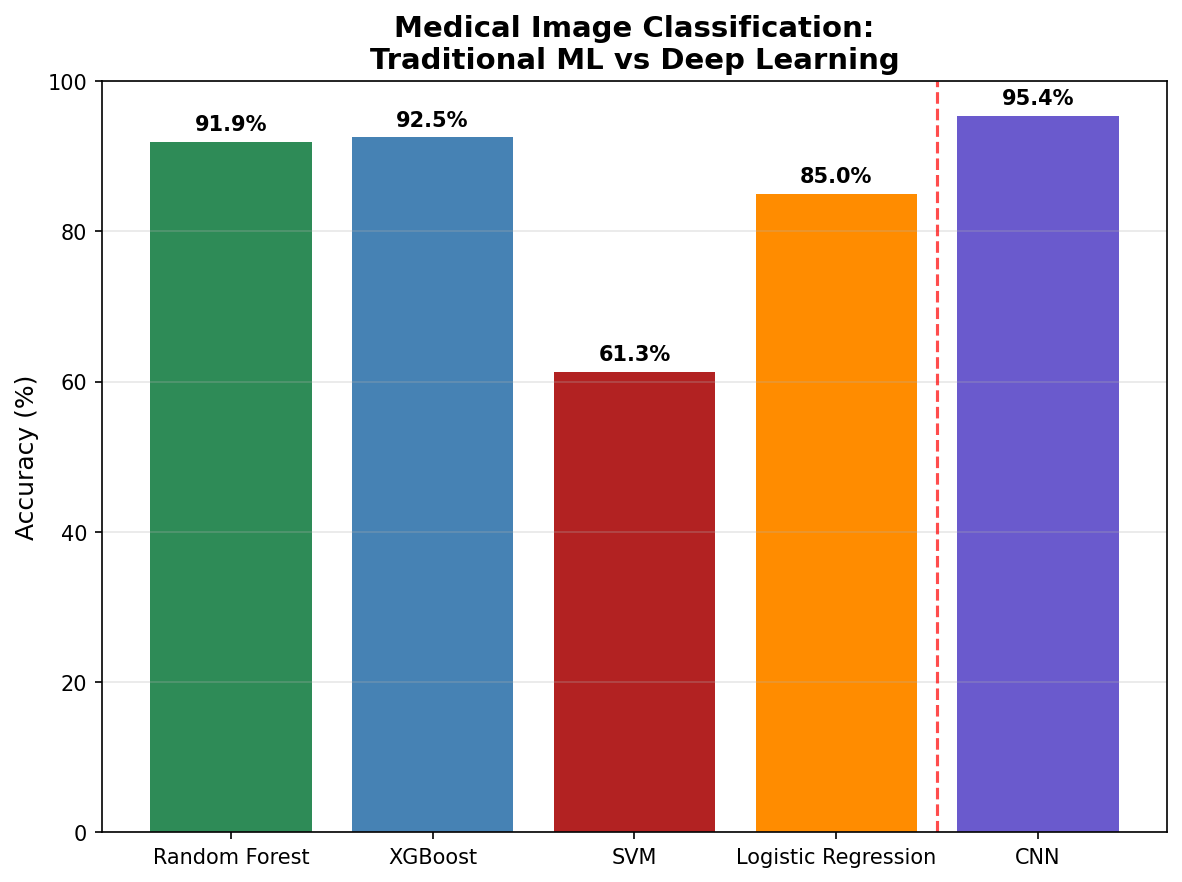
\includegraphics[width=0.8\textwidth]{images/ml_vs_cnn_comparison}
\caption{Final performance comparison: CNN vs traditional ML}
\label{fig:ml_vs_cnn_comparison}
\end{figure}

\begin{figure}[H]
\centering
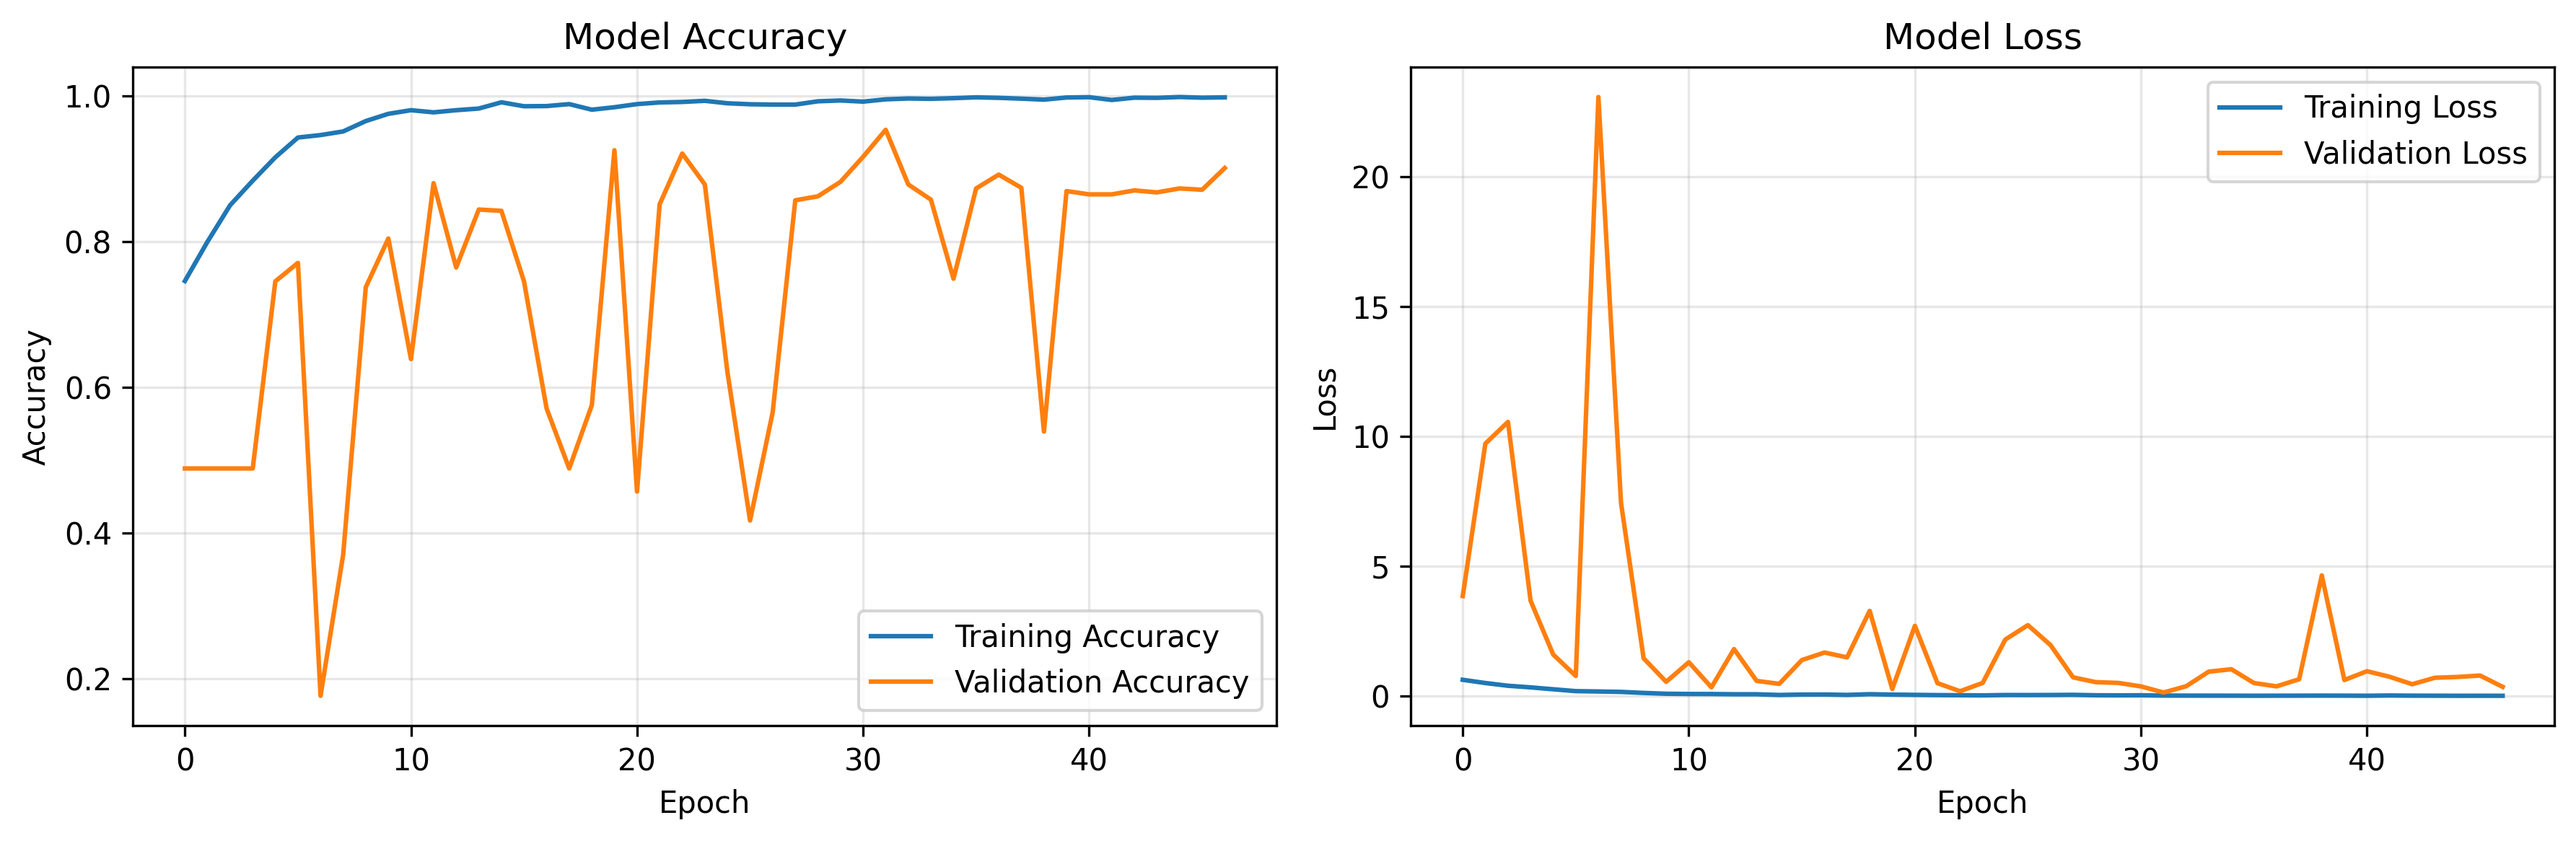
\includegraphics[width=0.8\textwidth]{images/nerthus_cnn_training_history}
\caption{CNN training history: accuracy and loss curves}
\label{fig:nerthus_cnn_training_history}
\end{figure}

\subsection{Statistical analysis}

\subsubsection{Cross-validation results}
Traditional ML models evaluated with 5-fold cross-validation:

\begin{table}[H]
\centering
\caption{Cross-validation performance (mean ± std)}
\begin{tabular}{lc}
\toprule
\textbf{Model} & \textbf{Accuracy} \\
\midrule
Random Forest & 0.935 ± 0.003 \\
XGBoost & 0.940 ± 0.014 \\
Logistic Regression & 0.812 ± 0.033 \\
\bottomrule
\end{tabular}
\end{table}

\subsubsection{Overfitting analysis}
CNN training showed controlled overfitting:
\begin{itemize}
    \item Final training accuracy: 99.8\%
    \item Best validation accuracy: 95.4\%
    \item Overfitting gap: 4.4\%
    \item Early stopping at epoch 47/200
\end{itemize}

\section{Technical implementation}

\subsection{Python package design}

\subsubsection{Class Architecture}
\begin{lstlisting}
class NerthusAnalyzer:
    """Main analysis pipeline"""
    def load_data(self): ...
    def analyze_image_features(self): ...
    def generate_report(self): ...

class NerthusML:
    """Traditional ML pipeline""" 
    def train_models(self): ...
    def robust_validation(self): ...
    def generate_report(self): ...

class NerthusCNN:
    """Deep learning pipeline"""
    def build_cnn(self): ...
    def train(self): ...
    def evaluate(self): ...
\end{lstlisting}

\subsubsection{Command line interface}
\begin{lstlisting}
# Complete pipeline (default values)
nerthus --cnn (--ml, --analysis, --processor)

# CNN
nerthus-cnn --help
python examples/nerthus_cnn_champion.py

# ML
nerthus-ml --help
python examples/nerthus_ml_pipeline.py

# Analysis
nerthus-analysis --help
examples/nerthus_image_analyzer.py

# Image processor
nerthus-processor --help
python examples/nerthus_image_processor.py

# Plot ML vs CNN comparison
python examples/nerthus_comparison_plot.py
\end{lstlisting}

\subsection{Code quality features}
\begin{itemize}
    \item Type hints and comprehensive docstrings
    \item Modular architecture with single responsibility
    \item Comprehensive error handling and logging
    \item Unit tests and validation scripts
    \item Professional documentation
\end{itemize}

\section{Web application implementation}
\label{sec:web_application}

This section describes the development and implementation of a fully functional web application that demonstrates the practical deployment of the Nerthus Medical ML pipeline for clinical use.

\subsection{Application architecture}

The web application is built using Streamlit, a Python framework designed for machine learning and data science applications. The architecture follows a modular design pattern for maintainability and extensibility.

\subsubsection{Technical stack}
\begin{itemize}
    \item \textbf{Frontend}: Streamlit with custom CSS styling
    \item \textbf{Backend}: Python with integrated model inference
    \item \textbf{Model serving}: Direct TensorFlow/Keras and Scikit-learn integration
    \item \textbf{Image processing}: OpenCV and PIL for medical image handling
\end{itemize}

\subsection{User interface design}

The application features a medical-grade interface designed for clinical usability:

\subsubsection{Dashboard overview}
\begin{itemize}
    \item Real-time model availability status
    \item Performance metrics visualization
    \item Project summary and clinical context
\end{itemize}

\subsubsection{Live prediction interface}
\begin{itemize}
    \item Drag-and-drop image upload functionality
    \item Model selection between CNN and ML
    \item Real-time BBPS scoring with confidence intervals
    \item Side-by-side model comparison when available
\end{itemize}

\subsubsection{Clinical reference materials}
\begin{itemize}
    \item Boston Bowel Preparation Scale (BBPS) reference guide
    \item Feature importance explanations
    \item Medical context and clinical significance
\end{itemize}

\subsection{Model integration}

The web application seamlessly integrates the trained machine learning models.

\subsubsection{Model loading system}
\begin{minted}{python}
class ModelLoader:
    def load_models(self, ml_path="XGBoost.joblib",
            cnn_path="CNN.keras"):
        # Load ML model
        self.ml_model = joblib.load(ml_path)
        # Load CNN with CPU fallback
        with tf.device('/CPU:0'):
            self.cnn_model = tf.keras.models.load_model(cnn_path)
    
    def extract_features_from_image(self, image)
    def predict_with_ml(self, image)
    def predict_with_cnn(self, image, debug=False)
\end{minted}

\subsection{Prediction workflow}

The prediction workflow follows clinical best practices:

\begin{enumerate}
    \item \textbf{Image upload}: User provides colonoscopy image via drag-and-drop interface
    \item \textbf{Preprocessing}: Automatic image validation and normalization
    \item \textbf{Feature extraction}: Computation of 22 medical image features
    \item \textbf{Model inference}: Parallel prediction using selected models
    \item \textbf{Result presentation}: BBPS score with confidence assessment
\end{enumerate}

\subsection{Error handling and validation}

Robust error handling ensures clinical reliability:

\subsubsection{Model fallback system}
\begin{itemize}
    \item Graceful degradation if models fail to load
    \item Clear error messages for clinical users
    \item Continued functionality with available models
\end{itemize}

\subsection{Performance characteristics}

\subsubsection{Response times}
\begin{table}[H]
\centering
\caption{Web application performance metrics}
\begin{tabular}{lcc}
\toprule
\textbf{Operation} & \textbf{Time (seconds)} & \textbf{Notes} \\
\midrule
Model loading & 2-5 & Initial application startup \\
Image upload & 1 & Client-side processing \\
Feature extraction & 1-2 & 22 medical features \\
ML prediction & 0.1 & Optimized inference \\
CNN prediction & 0.5-1 & CPU-based inference \\
Total response time & 2-4 & End-to-end prediction \\
\bottomrule
\end{tabular}
\end{table}

\subsubsection{Scalability considerations}
\begin{itemize}
    \item Stateless architecture supports multiple concurrent users
    \item Model caching for improved response times
    \item Memory-efficient image processing
\end{itemize}

\subsection{Clinical deployment considerations}

\subsubsection{Data privacy and security}
\begin{itemize}
    \item Local processing ensures no data transmission
    \item HIPAA-compliant (Health Insurance Portability and Accountability Act) architecture ready
    \item No persistent storage of medical images
\end{itemize}

\subsubsection{Integration with clinical workflows}
\begin{itemize}
    \item DICOM (Digital Imaging and Communications in Medicine) image format support ready for implementation
    \item EHR (Electronic Health Record) integration capabilities via API endpoints
    \item Export functionality for medical documentation
\end{itemize}

\subsubsection{User experience design}
\begin{itemize}
    \item Medical-grade color scheme and typography
    \item Intuitive navigation for clinical staff
    \item Accessibility considerations for diverse users
\end{itemize}

\subsection{Deployment options}

The web application supports multiple deployment scenarios:

\subsubsection{Local deployment}
\begin{verbatim}
cd web
pip install -r requirements.txt
streamlit run app.py / python run.py
\end{verbatim}

\subsubsection{Cloud deployment}
\begin{itemize}
    \item \textbf{Streamlit cloud}: Free tier for demonstration
    \item \textbf{Docker containerization}: Production deployment
    \item \textbf{Cloud platforms}: AWS, Azure, GCP compatibility
\end{itemize}

\subsubsection{Enterprise deployment}
\begin{itemize}
    \item Hospital network installation
    \item Multi-user authentication systems
    \item Audit logging for clinical use
\end{itemize}

\subsection{Clinical validation}

The web application uses the same validated models and features as the research pipeline:

\begin{itemize}
    \item \textbf{Model accuracy}: 95.4\% (CNN) and 92.5\% (ML)
    \item \textbf{Feature consistency}: Identical 22-feature extraction
    \item \textbf{Preprocessing pipeline}: Matches training methodology
\end{itemize}

\subsection{Future enhancements}

Potential enhancements for clinical production use:

\begin{itemize}
    \item Real-time video stream processing
    \item Multi-frame temporal analysis
    \item Integration with endoscopic reporting systems
    \item Quality metrics dashboard for procedure analytics
\end{itemize}

The web application successfully demonstrates the translation of machine learning research into a practical clinical tool, providing immediate value for bowel preparation quality assessment while maintaining the rigorous validation standards of the underlying research.

\section{Discussion}

\subsection{Performance insights}

\subsubsection{Traditional ML strengths}
\begin{itemize}
    \item \textbf{92.5\% accuracy} with handcrafted features
    \item Fast training and inference (3 minutes)
    \item Interpretable feature importance
    \item Stable performance across runs
\end{itemize}

\subsubsection{Deep Learning advantages}
\begin{itemize}
    \item \textbf{95.4\% accuracy} learning from raw pixels
    \item Automatic feature extraction
    \item State-of-the-art approach
    \item Potential for further improvement
\end{itemize}

\subsection{Limitations and challenges}

\subsubsection{Technical challenges}
\begin{itemize}
    \item CNN training instability and overfitting
    \item Computational requirements for deep learning
    \item Hyperparameter sensitivity in neural networks
\end{itemize}

\subsubsection{Medical considerations}
\begin{itemize}
    \item Single-center dataset limitation
    \item Need for multi-rater ground truth validation
    \item Clinical deployment requirements
\end{itemize}

\section{Conclusion and future work}

\subsection{Key conclusions}
\begin{enumerate}
    \item \textbf{CNN achieves superior performance} (95.4\%) for medical image classification
    \item \textbf{Systematic optimization} is crucial for deep learning success
    \item \textbf{Both approaches have merits} for different deployment scenarios
    \item \textbf{Production-ready implementation} demonstrates professional ML engineering skills
\end{enumerate}

\subsection{Future directions}

\subsubsection{Technical enhancements}
\begin{itemize}
    \item Transfer learning with medical pre-trained models
    \item Ensemble methods combining ML and DL approaches
    \item Explainable AI for clinical interpretability
    \item Real-time inference optimization
\end{itemize}

\subsubsection{Medical applications}
\begin{itemize}
    \item Multi-center validation studies
    \item Integration with endoscopic reporting systems
    \item Real-time quality assessment during procedures
    \item Regulatory approval pathway development
\end{itemize}

\section*{Acknowledgments}

The Nerthus dataset was created by Pogorelov et al. and hosted on Kaggle. This project builds upon their valuable contribution to medical AI research.

\subsection*{Dataset citation}
\begin{verbatim}
@inproceedings{Pogorelov:2017:NBP,
  author = {Pogorelov, Konstantin and Randel, Kristin Ranheim and 
            de Lange, Thomas and Eskeland, Sigrun Losada and 
            Griwodz, Carsten and Johansen, Dag and 
            Spampinato, Concetto and Taschwer, Mario and 
            Lux, Mathias and Schmidt, Peter Thelin and 
            Riegler, Michael and Halvorsen, Pal},
  title = {Nerthus: A Bowel Preparation Quality Video Dataset},
  booktitle = {Proceedings of the 8th ACM on Multimedia Systems Conference},
  year = {2017},
  pages = {170--174}
}
\end{verbatim}

\appendix
\section{Appendix}
\label{app:appendix}

This appendix provides detailed descriptions of the 22 medical image features extracted for bowel preparation quality assessment, including their mathematical definitions, units, and clinical relevance. It also describes the Python project structure.

\section{Medical image feature descriptions}
\label{app:feature_descriptions}

\subsection{Texture features (GLCM)}

Texture features are computed from the Gray Level Co-occurrence Matrix (GLCM), which captures spatial relationships between pixel intensities.

\subsubsection{Contrast}
\begin{itemize}
    \item \textbf{Definition}: Measures local intensity variations and sharp transitions
    \item \textbf{Formula}: $\displaystyle \sum_{i,j} |i-j|^2 \cdot P(i,j)$ where $P(i,j)$ is the co-occurrence probability
    \item \textbf{Units}: Unitless (higher values indicate more contrast)
    \item \textbf{Medical Relevance}: High contrast suggests clear mucosal boundaries in well-prepared bowels
\end{itemize}

\subsubsection{Homogeneity (Inverse difference moment)}
\begin{itemize}
    \item \textbf{Definition}: Measures uniformity and smoothness of texture
    \item \textbf{Formula}: $\displaystyle \sum_{i,j} \frac{P(i,j)}{1 + |i-j|}$
    \item \textbf{Units}: Unitless (0 to 1, where 1 = perfectly homogeneous)
    \item \textbf{Medical Relevance}: High homogeneity indicates smooth mucosal surfaces
\end{itemize}

\subsubsection{Energy (Angular second moment)}
\begin{itemize}
    \item \textbf{Definition}: Measures textural uniformity and pattern repetition
    \item \textbf{Formula}: $\displaystyle \sum_{i,j} P(i,j)^2$
    \item \textbf{Units}: Unitless (0 to 1, where 1 = perfectly uniform)
    \item \textbf{Medical Relevance}: High energy suggests regular tissue patterns
\end{itemize}

\subsubsection{Correlation}
\begin{itemize}
    \item \textbf{Definition}: Measures linear dependency of gray levels on neighboring pixels
    \item \textbf{Formula}: $\displaystyle \sum_{i,j} \frac{(i-\mu_i)(j-\mu_j)P(i,j)}{\sigma_i\sigma_j}$
    \item \textbf{Units}: Unitless (-1 to 1)
    \item \textbf{Medical Relevance}: High correlation indicates structured tissue patterns
\end{itemize}

\subsection{Color space features}

Color features analyze tissue appearance in different color spaces to distinguish between mucosa and residual materials.

\subsubsection{Hue mean (HSV color space)}
\begin{itemize}
    \item \textbf{Definition}: Average dominant color tone (red, green, blue, etc.)
    \item \textbf{Range}: 0° to 360° (normalized to 0-1 in processing)
    \item \textbf{Units}: Degrees or normalized (0-1)
    \item \textbf{Medical Relevance}: Differentiates pinkish mucosa from brown/green stool
\end{itemize}

\subsubsection{Saturation mean (HSV color space)}
\begin{itemize}
    \item \textbf{Definition}: Average color purity and intensity
    \item \textbf{Range}: 0 to 1 (0 = grayscale, 1 = fully saturated)
    \item \textbf{Units}: Unitless (0-1)
    \item \textbf{Medical Relevance}: High saturation indicates vivid mucosal colors
\end{itemize}

\subsubsection{Value mean (HSV color space)}
\begin{itemize}
    \item \textbf{Definition}: Average brightness or lightness
    \item \textbf{Range}: 0 to 1 (0 = black, 1 = white)
    \item \textbf{Units}: Unitless (0-1)
    \item \textbf{Medical Relevance}: Indicates illumination quality and tissue visibility
\end{itemize}

\subsubsection{L* mean (LAB color space)}
\begin{itemize}
    \item \textbf{Definition}: Perceptual lightness (designed for human vision)
    \item \textbf{Range}: 0 to 100 (0 = black, 100 = white)
    \item \textbf{Units}: Lightness units
    \item \textbf{Medical Relevance}: Correlates with human perception of tissue brightness
\end{itemize}

\subsubsection{a* mean (LAB color space)}
\begin{itemize}
    \item \textbf{Definition}: Position between red/magenta and green
    \item \textbf{Range}: -128 to 127 (negative = green, positive = red)
    \item \textbf{Units}: Color difference units
    \item \textbf{Medical Relevance}: Positive values indicate reddish mucosal tissue
\end{itemize}

\subsubsection{b* mean (LAB color space)}
\begin{itemize}
    \item \textbf{Definition}: Position between blue and yellow
    \item \textbf{Range}: -128 to 127 (negative = blue, positive = yellow)
    \item \textbf{Units}: Color difference units
    \item \textbf{Medical Relevance}: Positive values indicate yellowish stool or bile
\end{itemize}

\subsection{Edge and shape features}

Edge features capture anatomical structures and detail visibility.

\subsubsection{Edge density}
\begin{itemize}
    \item \textbf{Definition}: Proportion of edge pixels in the image
    \item \textbf{Formula}: $\displaystyle \frac{\text{Number of edge pixels}}{\text{Total pixels}}$
    \item \textbf{Units}: Unitless ratio (0 to 1)
    \item \textbf{Medical Relevance}: High density indicates detailed mucosal patterns
\end{itemize}

\subsubsection{Sharpness}
\begin{itemize}
    \item \textbf{Definition}: Focus quality measured by Laplacian variance
    \item \textbf{Formula}: $\text{Var}(\nabla^2 I)$ where $\nabla^2$ is the Laplacian operator
    \item \textbf{Units}: Pixel intensity variance squared
    \item \textbf{Medical Relevance}: High sharpness indicates clear, well-focused images
\end{itemize}

\subsection{Intensity statistics}

Intensity features capture overall brightness characteristics and variations.

\subsubsection{Mean intensity}
\begin{itemize}
    \item \textbf{Definition}: Average pixel intensity
    \item \textbf{Formula}: $\displaystyle \frac{1}{N}\sum_{i=1}^N I_i$
    \item \textbf{Units}: Pixel intensity (0-255 for 8-bit images)
    \item \textbf{Medical Relevance}: Overall tissue brightness and illumination
\end{itemize}

\subsubsection{Standard deviation intensity}
\begin{itemize}
    \item \textbf{Definition}: Measure of intensity variation
    \item \textbf{Formula}: $\displaystyle \sqrt{\frac{1}{N}\sum_{i=1}^N (I_i - \mu)^2}$
    \item \textbf{Units}: Pixel intensity
    \item \textbf{Medical Relevance}: High values indicate good contrast and detail
\end{itemize}

\subsubsection{Minimum intensity}
\begin{itemize}
    \item \textbf{Definition}: Darkest pixel value in the image
    \item \textbf{Units}: Pixel intensity (0-255)
    \item \textbf{Medical Relevance}: Represents shadows or dark residue
\end{itemize}

\subsubsection{Maximum intensity}
\begin{itemize}
    \item \textbf{Definition}: Brightest pixel value in the image
    \item \textbf{Units}: Pixel intensity (0-255)
    \item \textbf{Medical Relevance}: Represents specular highlights or well-lit areas
\end{itemize}

\subsubsection{Median intensity}
\begin{itemize}
    \item \textbf{Definition}: Middle value of sorted pixel intensities
    \item \textbf{Units}: Pixel intensity (0-255)
    \item \textbf{Medical Relevance}: Robust measure of typical tissue brightness
\end{itemize}

\subsection{Advanced texture features}

Advanced features capture complex patterns and micro-textures.

\subsubsection{Image entropy}
\begin{itemize}
    \item \textbf{Definition}: Measure of randomness and complexity
    \item \textbf{Formula}: $\displaystyle -\sum_{i=1}^N p(i) \log_2 p(i)$ where $p(i)$ is intensity probability
    \item \textbf{Units}: Bits (information theory)
    \item \textbf{Medical Relevance}: High entropy indicates complex tissue patterns
\end{itemize}

\subsubsection{LBP entropy (Local binary patterns)}
\begin{itemize}
    \item \textbf{Definition}: Entropy of local texture patterns
    \item \textbf{Units}: Bits
    \item \textbf{Medical Relevance}: Captures micro-texture variations in mucosa
\end{itemize}

\subsubsection{Blob count}
\begin{itemize}
    \item \textbf{Definition}: Number of connected components in edge map
    \item \textbf{Units}: Count (integer)
    \item \textbf{Medical Relevance}: Many blobs indicate particulate matter or detailed structures
\end{itemize}

\subsection{Clinical interpretation by BBPS score}

\begin{table}[H]
\centering
\caption{Typical feature patterns by Bowel preparation quality}
\begin{tabular}{p{3cm}p{4cm}p{4cm}p{4cm}}
\toprule
\textbf{Feature Category} & \textbf{BBPS 3 (Excellent)} & \textbf{BBPS 2 (Good)} & \textbf{BBPS 0-1 (Poor)} \\
\midrule
\textbf{Texture} & High contrast, medium homogeneity & Moderate contrast & Low contrast, high homogeneity \\
\textbf{Color} & Appropriate hue (pinkish-red) & Slight color deviation & Abnormal colors (brown/green) \\
\textbf{Edges} & High edge density, high sharpness & Reduced edge density & Very low edge density \\
\textbf{Intensity} & Good dynamic range & Some intensity loss & Poor dynamic range \\
\textbf{Entropy} & Medium-high complexity & Reduced complexity & Low complexity \\
\bottomrule
\end{tabular}
\end{table}

\subsubsection{BBPS 3 (Excellent preparation)}
\begin{itemize}
    \item High edge density and sharpness
    \item Appropriate mucosal colors (pinkish-red hues)
    \item Complex texture patterns (medium-high entropy)
    \item Good contrast and intensity range
\end{itemize}

\subsubsection{BBPS 2 (Good preparation)}
\begin{itemize}
    \item Moderate edge density with some detail loss
    \item Slight color deviation from ideal
    \item Reduced texture complexity
    \item Acceptable but not optimal sharpness
\end{itemize}

\subsubsection{BBPS 1 (Poor preparation)}
\begin{itemize}
    \item Low edge density with obscured details
    \item Significant color staining
    \item Homogeneous textures (low entropy)
    \item Poor sharpness and contrast
\end{itemize}

\subsubsection{BBPS 0 (Unprepared)}
\begin{itemize}
    \item Very low edge density (completely obscured)
    \item Extreme color deviation (solid stool)
    \item Very simple textures
    \item Minimal visible mucosal patterns
\end{itemize}

\subsection{Feature selection rationale}

These 22 features were selected because they collectively capture:

\begin{itemize}
    \item \textbf{Macro-texture}: Large-scale tissue patterns (GLCM features)
    \item \textbf{Micro-texture}: Fine details and complexity (entropy, LBP)
    \item \textbf{Color characteristics}: Tissue appearance vs. residual materials
    \item \textbf{Structural details}: Anatomical visibility (edge features)
    \item \textbf{Overall quality}: Illumination and focus (intensity statistics)
\end{itemize}

The combination of these diverse feature types enables robust differentiation between preparation quality levels, as demonstrated by the 92.5\%-95.4\% classification accuracy achieved in this project.


\section{Project}

\subsection{Project structure details}

Complete file structure of the Nerthus Medical ML project:

\begin{lstlisting}
nerthus-medical-ml/
|-- AUTHORS.txt					# Author(s)
|-- examples
|   |-- nerthus_cnn_champion.py
|   |-- nerthus_cnn_improved.py
|   |-- nerthus_cnn_simple.py
|   |-- nerthus_cnn_tuning.py
|   |-- nerthus_comparison_plot.py
|   |-- nerthus_image_analyzer.py
|   |-- nerthus_image_processor.py
|   `-- nerthus_ml_pipeline.py
|-- nerthus
|   |-- analyzer.py				# Data analysis & EDA
|   |-- cli.py					# Command line interface
|   |-- cnn.py					# Deep learning
|   |-- __init__.py
|   |-- ml.py					# Traditional ML
|   |-- processor.py				# Image processing
|   `-- utils.py				# Utilities
|-- pyproject.toml				# Modern Python packaging
|-- README.md					# Project description
|-- report
|   |-- images					# Visualization files
|   |-- Makefile				# Building the report
|   |-- Report.pdf				# Report PDF file
|   |-- Report.tex				# Report LateX file
|   `-- requirements.sh				# Prerequisites for the report
|-- requirements.txt				# Python project requirements
|-- setup.py					# Setup file
`-- web
    |-- app.py					# Web app file
    |-- debug_cnn.py				# CNN debug file
    |-- loader.py				# Model loader
    |-- requirements.txt			# Web app requirements
    |-- run.py					# Run web app with Python
    |-- static					# Static file for the web app
    `-- utils.py				# Web app utilities
\end{lstlisting}

\subsection{Model configuration details}

\subsubsection{Optimal CNN hyperparameters}
\begin{itemize}
    \item \textbf{Dropout rates}: [0.1, 0.2, 0.3, 0.2]
    \item \textbf{Batch size}: 32
    \item \textbf{Learning rate}: 0.001 with reduction on plateau
    \item \textbf{Early stopping}: Patience of 15 epochs
    \item \textbf{Input shape}: 150x150x3
\end{itemize}

\subsubsection{ML parameters}
\begin{itemize}
    \item \textbf{n\_estimators}: 100
    \item \textbf{max\_depth}: None (unlimited)
    \item \textbf{random\_state}: 42
    \item \textbf{n\_jobs}: -1 (use all cores, CPU-based)
\end{itemize}

\subsection{ML confusion matrix}
\begin{figure}[H]
\centering
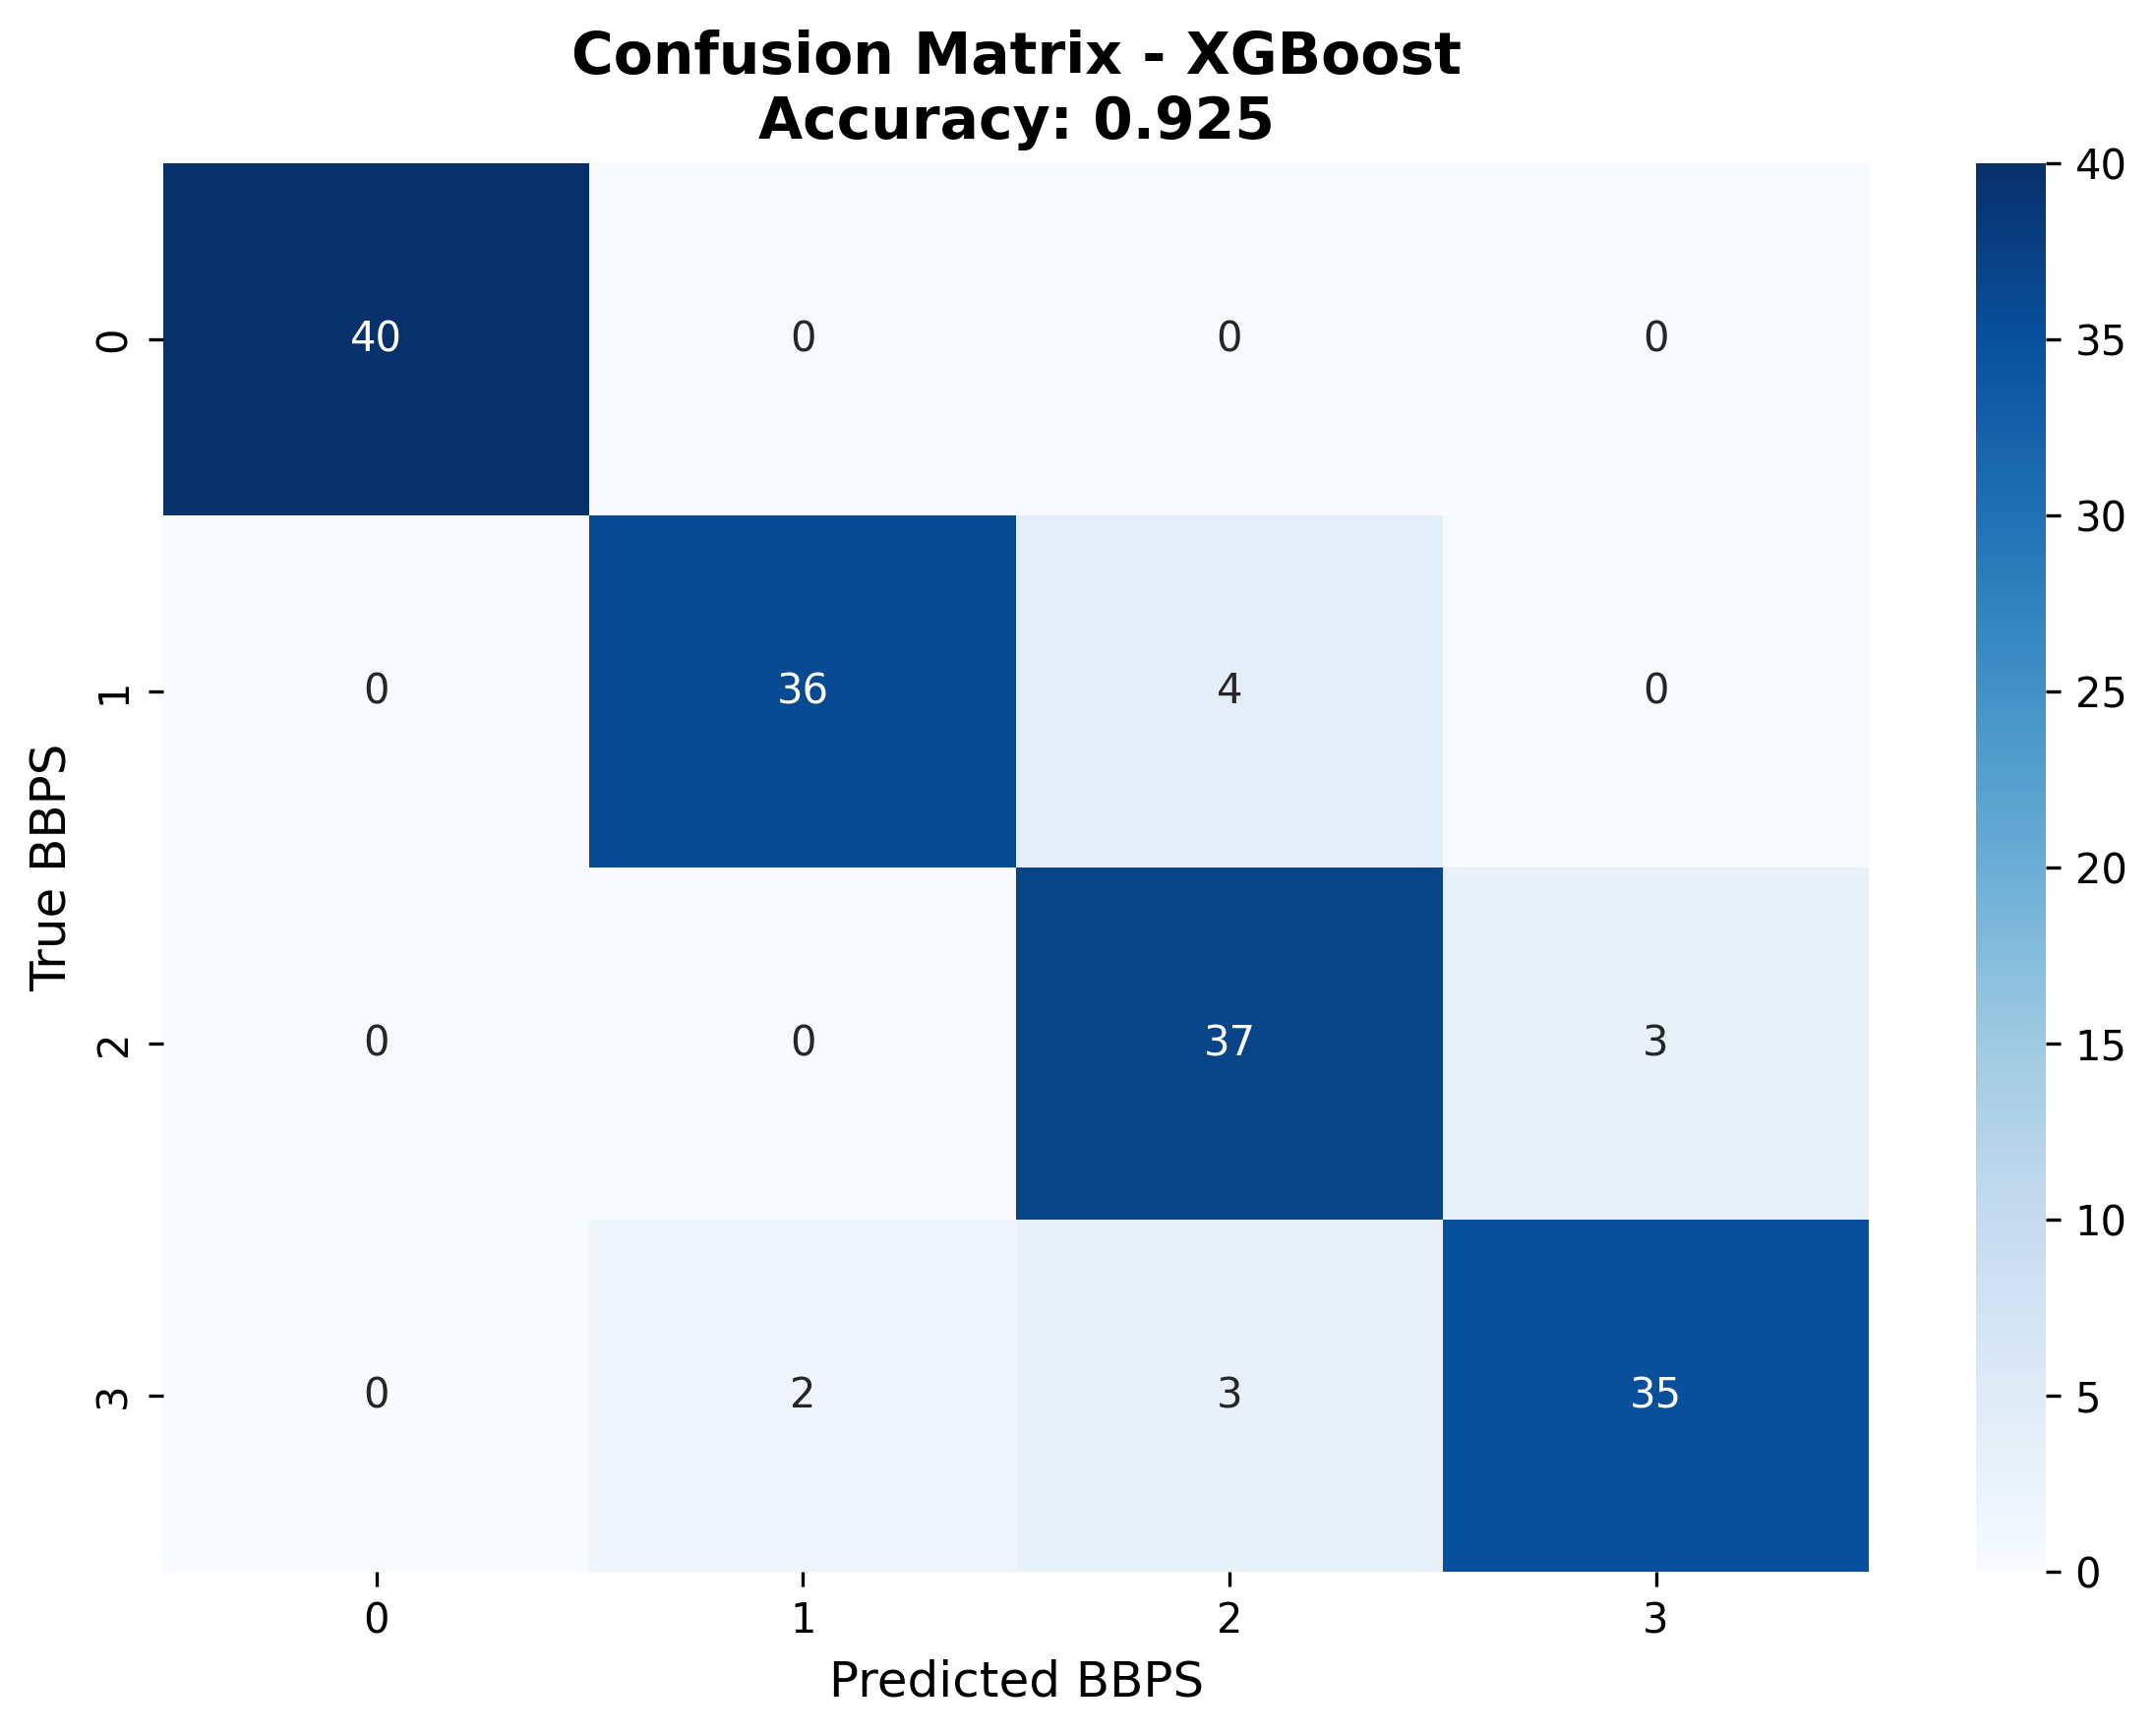
\includegraphics[width=0.8\textwidth]{images/confusion_matrix_xgboost}
\caption{Confusion matrix XGBoost}
\label{fig:confusion_matrix_xgboost}
\end{figure}

\begin{figure}[H]
\centering
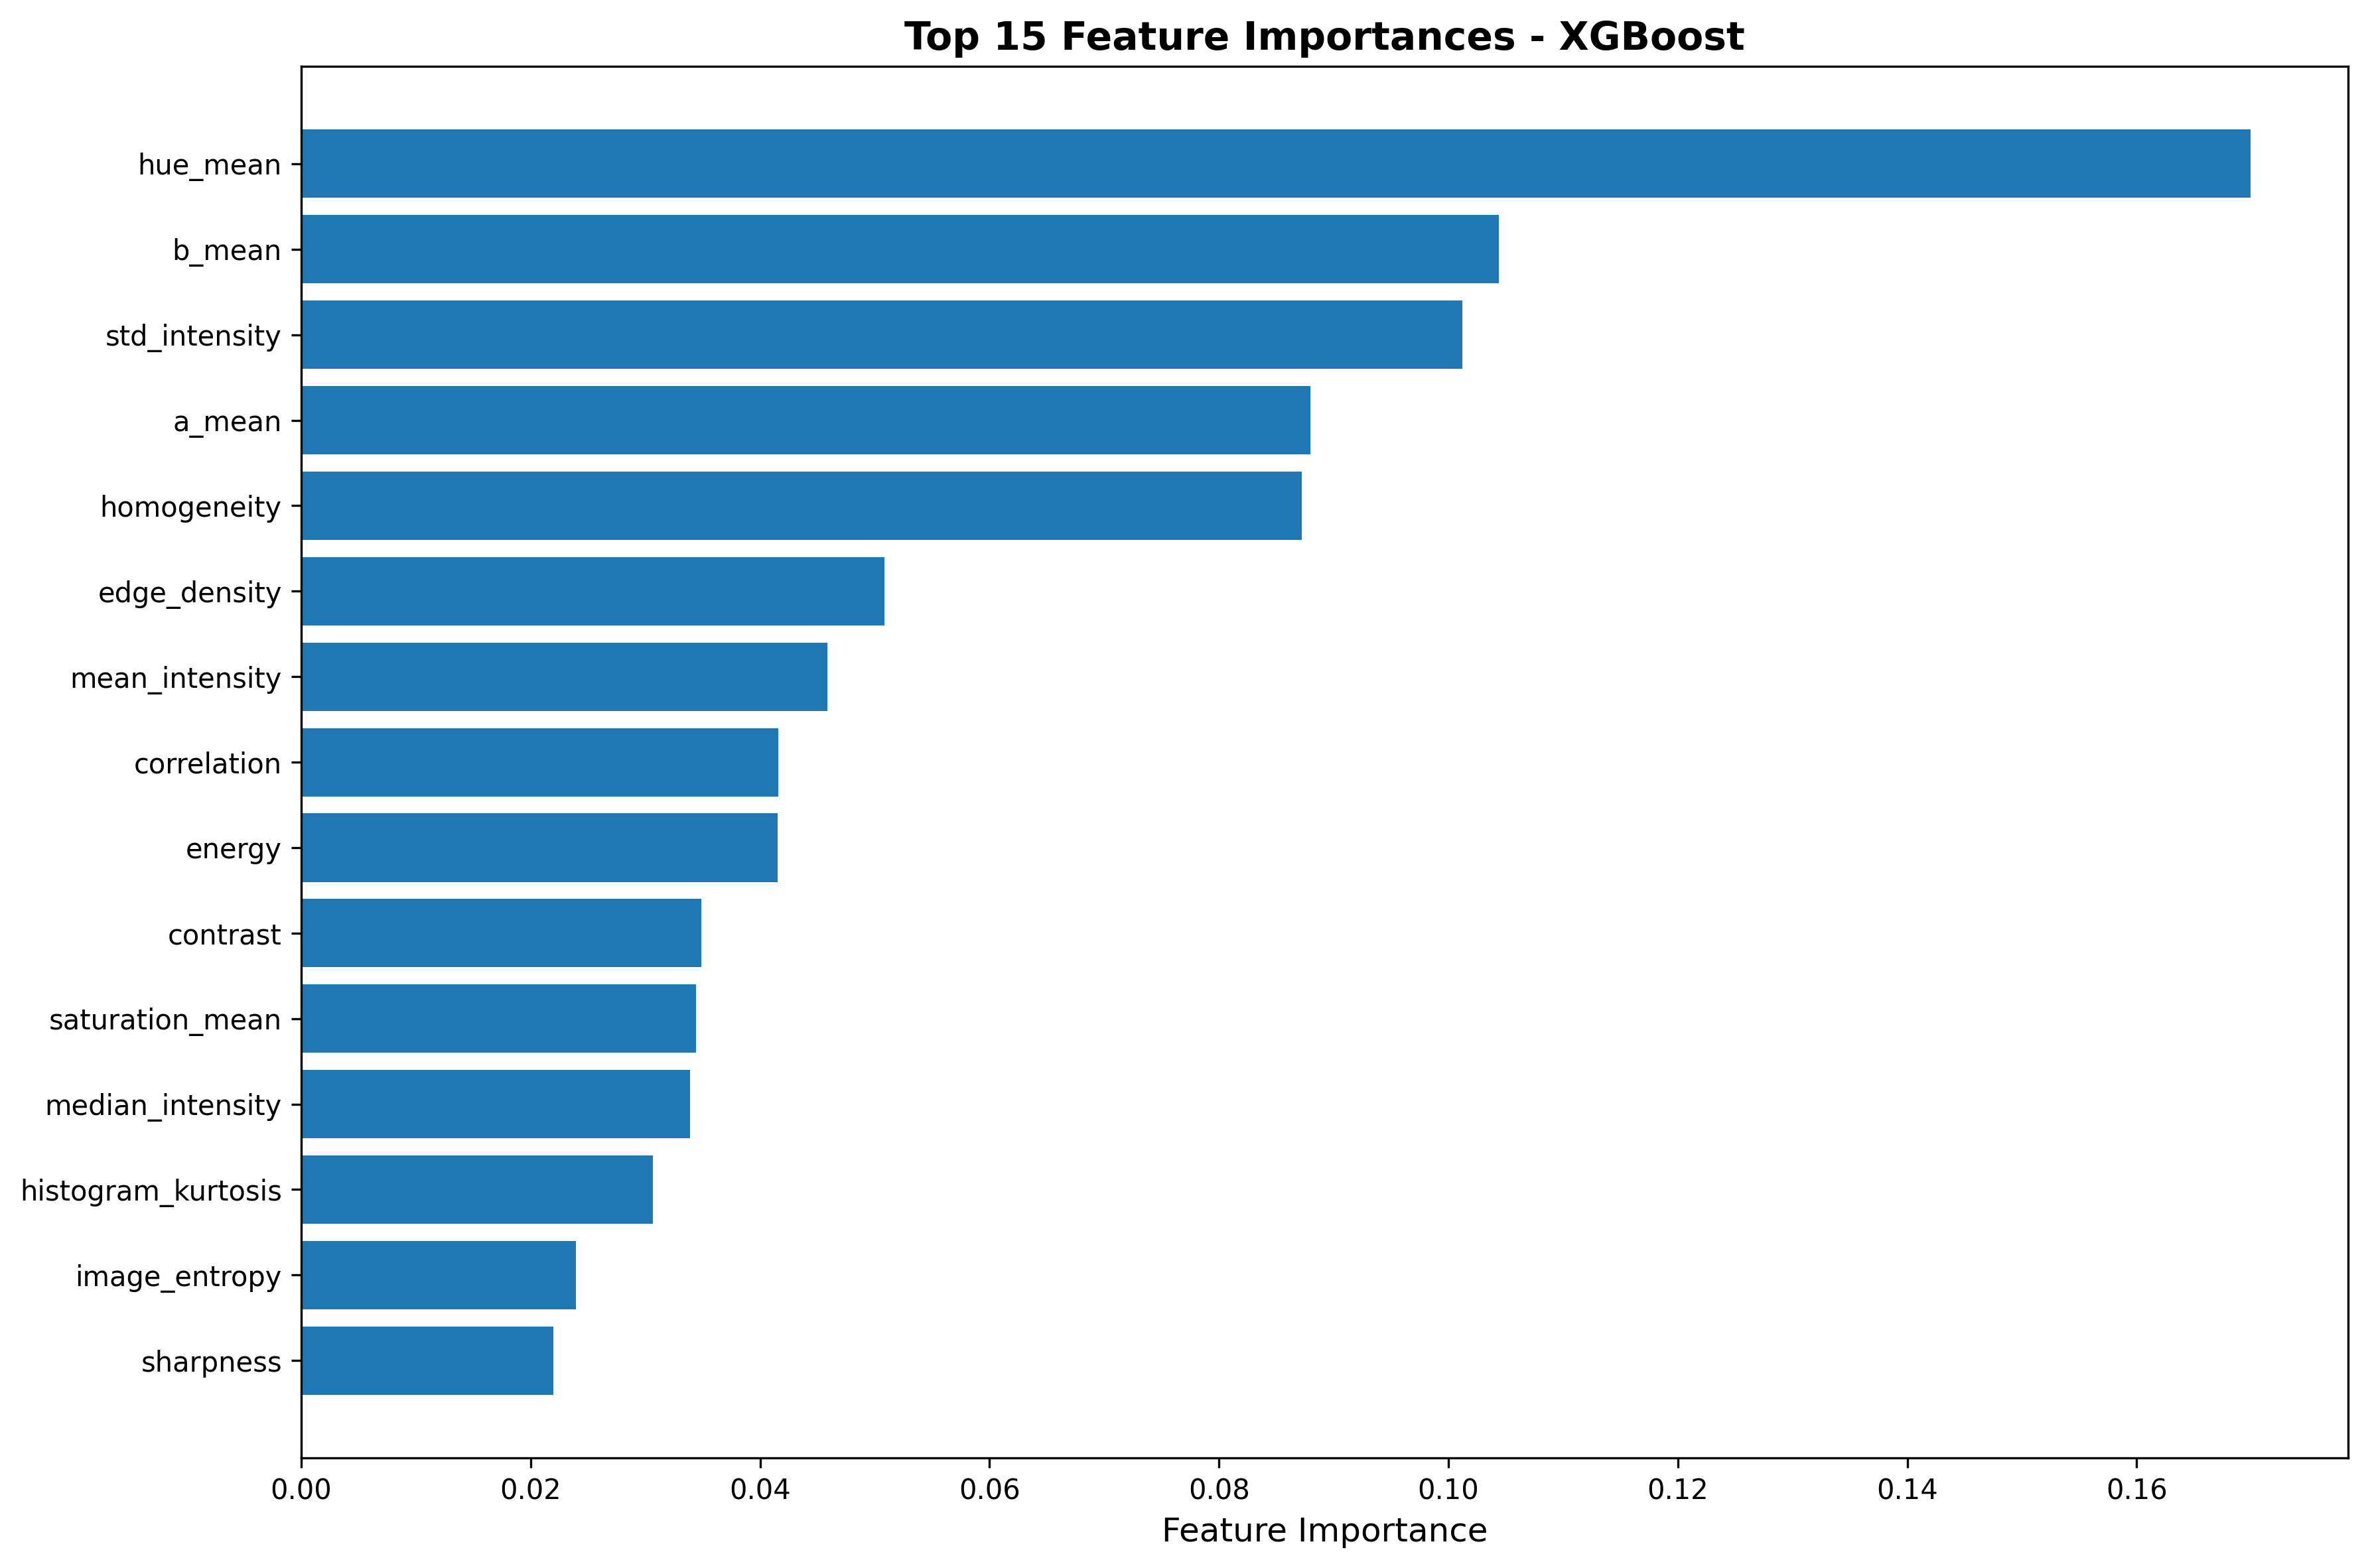
\includegraphics[width=0.8\textwidth]{images/feature_importance_xgboost}
\caption{Feature importance XGBoost}
\label{fig:feature_importance_xgboost}
\end{figure}

\end{document}
